\documentclass[twoside]{book}

% Packages required by doxygen
\usepackage{fixltx2e}
\usepackage{calc}
\usepackage{doxygen}
\usepackage[export]{adjustbox} % also loads graphicx
\usepackage{graphicx}
\usepackage[utf8]{inputenc}
\usepackage{makeidx}
\usepackage{multicol}
\usepackage{multirow}
\PassOptionsToPackage{warn}{textcomp}
\usepackage{textcomp}
\usepackage[nointegrals]{wasysym}
\usepackage[table]{xcolor}

% Font selection
\usepackage[T1]{fontenc}
\usepackage[scaled=.90]{helvet}
\usepackage{courier}
\usepackage{amssymb}
\usepackage{sectsty}
\renewcommand{\familydefault}{\sfdefault}
\allsectionsfont{%
  \fontseries{bc}\selectfont%
  \color{darkgray}%
}
\renewcommand{\DoxyLabelFont}{%
  \fontseries{bc}\selectfont%
  \color{darkgray}%
}
\newcommand{\+}{\discretionary{\mbox{\scriptsize$\hookleftarrow$}}{}{}}

% Page & text layout
\usepackage{geometry}
\geometry{%
  a4paper,%
  top=2.5cm,%
  bottom=2.5cm,%
  left=2.5cm,%
  right=2.5cm%
}
\tolerance=750
\hfuzz=15pt
\hbadness=750
\setlength{\emergencystretch}{15pt}
\setlength{\parindent}{0cm}
\setlength{\parskip}{3ex plus 2ex minus 2ex}
\makeatletter
\renewcommand{\paragraph}{%
  \@startsection{paragraph}{4}{0ex}{-1.0ex}{1.0ex}{%
    \normalfont\normalsize\bfseries\SS@parafont%
  }%
}
\renewcommand{\subparagraph}{%
  \@startsection{subparagraph}{5}{0ex}{-1.0ex}{1.0ex}{%
    \normalfont\normalsize\bfseries\SS@subparafont%
  }%
}
\makeatother

% Headers & footers
\usepackage{fancyhdr}
\pagestyle{fancyplain}
\fancyhead[LE]{\fancyplain{}{\bfseries\thepage}}
\fancyhead[CE]{\fancyplain{}{}}
\fancyhead[RE]{\fancyplain{}{\bfseries\leftmark}}
\fancyhead[LO]{\fancyplain{}{\bfseries\rightmark}}
\fancyhead[CO]{\fancyplain{}{}}
\fancyhead[RO]{\fancyplain{}{\bfseries\thepage}}
\fancyfoot[LE]{\fancyplain{}{}}
\fancyfoot[CE]{\fancyplain{}{}}
\fancyfoot[RE]{\fancyplain{}{\bfseries\scriptsize Generated by Doxygen }}
\fancyfoot[LO]{\fancyplain{}{\bfseries\scriptsize Generated by Doxygen }}
\fancyfoot[CO]{\fancyplain{}{}}
\fancyfoot[RO]{\fancyplain{}{}}
\renewcommand{\footrulewidth}{0.4pt}
\renewcommand{\chaptermark}[1]{%
  \markboth{#1}{}%
}
\renewcommand{\sectionmark}[1]{%
  \markright{\thesection\ #1}%
}

% Indices & bibliography
\usepackage{natbib}
\usepackage[titles]{tocloft}
\setcounter{tocdepth}{3}
\setcounter{secnumdepth}{5}
\makeindex

% Hyperlinks (required, but should be loaded last)
\usepackage{ifpdf}
\ifpdf
  \usepackage[pdftex,pagebackref=true]{hyperref}
\else
  \usepackage[ps2pdf,pagebackref=true]{hyperref}
\fi
\hypersetup{%
  colorlinks=true,%
  linkcolor=blue,%
  citecolor=blue,%
  unicode%
}

% Custom commands
\newcommand{\clearemptydoublepage}{%
  \newpage{\pagestyle{empty}\cleardoublepage}%
}

\usepackage{caption}
\captionsetup{labelsep=space,justification=centering,font={bf},singlelinecheck=off,skip=4pt,position=top}

%===== C O N T E N T S =====

\begin{document}

% Titlepage & ToC
\hypersetup{pageanchor=false,
             bookmarksnumbered=true,
             pdfencoding=unicode
            }
\pagenumbering{roman}
\begin{titlepage}
\vspace*{7cm}
\begin{center}%
{\Large P\+A05 }\\
\vspace*{1cm}
{\large Generated by Doxygen 1.8.11}\\
\end{center}
\end{titlepage}
\clearemptydoublepage
\tableofcontents
\clearemptydoublepage
\pagenumbering{arabic}
\hypersetup{pageanchor=true}

%--- Begin generated contents ---
\chapter{Hierarchical Index}
\section{Class Hierarchy}
This inheritance list is sorted roughly, but not completely, alphabetically\+:\begin{DoxyCompactList}
\item \contentsline{section}{Event}{\pageref{struct_event}}{}
\item \contentsline{section}{Event\+Queue}{\pageref{class_event_queue}}{}
\begin{DoxyCompactList}
\item \contentsline{section}{A\+B\+Event\+Queue}{\pageref{class_a_b_event_queue}}{}
\item \contentsline{section}{L\+L\+Event\+Queue}{\pageref{class_l_l_event_queue}}{}
\end{DoxyCompactList}
\item \contentsline{section}{L\+L\+E\+Q\+Node}{\pageref{struct_l_l_e_q_node}}{}
\item \contentsline{section}{Teller\+Setup}{\pageref{class_teller_setup}}{}
\begin{DoxyCompactList}
\item \contentsline{section}{Teller\+Setup\+\_\+1\+QnT}{\pageref{class_teller_setup__1_qn_t}}{}
\item \contentsline{section}{Teller\+Setup\+\_\+n\+QnT}{\pageref{class_teller_setup__n_qn_t}}{}
\end{DoxyCompactList}
\item \contentsline{section}{Tickable}{\pageref{class_tickable}}{}
\begin{DoxyCompactList}
\item \contentsline{section}{Teller}{\pageref{class_teller}}{}
\item \contentsline{section}{Tickable\+Queue}{\pageref{class_tickable_queue}}{}
\end{DoxyCompactList}
\end{DoxyCompactList}

\chapter{Class Index}
\section{Class List}
Here are the classes, structs, unions and interfaces with brief descriptions\+:\begin{DoxyCompactList}
\item\contentsline{section}{\hyperlink{class_a_b_event_queue}{A\+B\+Event\+Queue} \\*An Array-\/\+Based \hyperlink{struct_event}{Event} Queue }{\pageref{class_a_b_event_queue}}{}
\item\contentsline{section}{\hyperlink{struct_event}{Event} }{\pageref{struct_event}}{}
\item\contentsline{section}{\hyperlink{class_event_queue}{Event\+Queue} }{\pageref{class_event_queue}}{}
\item\contentsline{section}{\hyperlink{struct_l_l_e_q_node}{L\+L\+E\+Q\+Node} \\*A node in an \hyperlink{class_l_l_event_queue}{L\+L\+Event\+Queue} }{\pageref{struct_l_l_e_q_node}}{}
\item\contentsline{section}{\hyperlink{class_l_l_event_queue}{L\+L\+Event\+Queue} \\*A Linked-\/\+List-\/\+Based \hyperlink{struct_event}{Event} Queue }{\pageref{class_l_l_event_queue}}{}
\item\contentsline{section}{\hyperlink{class_teller}{Teller} \\*Models a bank teller }{\pageref{class_teller}}{}
\item\contentsline{section}{\hyperlink{class_teller_setup}{Teller\+Setup} }{\pageref{class_teller_setup}}{}
\item\contentsline{section}{\hyperlink{class_teller_setup__1_qn_t}{Teller\+Setup\+\_\+1\+QnT} }{\pageref{class_teller_setup__1_qn_t}}{}
\item\contentsline{section}{\hyperlink{class_teller_setup__n_qn_t}{Teller\+Setup\+\_\+n\+QnT} }{\pageref{class_teller_setup__n_qn_t}}{}
\item\contentsline{section}{\hyperlink{class_tickable}{Tickable} \\*A \hyperlink{class_tickable}{Tickable} object }{\pageref{class_tickable}}{}
\item\contentsline{section}{\hyperlink{class_tickable_queue}{Tickable\+Queue} \\*An \hyperlink{class_event_queue}{Event\+Queue} wrapper that enables tick functionality }{\pageref{class_tickable_queue}}{}
\end{DoxyCompactList}

\chapter{File Index}
\section{File List}
Here is a list of all documented files with brief descriptions\+:\begin{DoxyCompactList}
\item\contentsline{section}{\hyperlink{PA02_8cpp}{P\+A02.\+cpp} \\*Implements the program entry point }{\pageref{PA02_8cpp}}{}
\end{DoxyCompactList}

\chapter{Class Documentation}
\hypertarget{class_a_b_event_queue}{}\section{A\+B\+Event\+Queue Class Reference}
\label{class_a_b_event_queue}\index{A\+B\+Event\+Queue@{A\+B\+Event\+Queue}}


An Array-\/\+Based \hyperlink{struct_event}{Event} Queue.  




{\ttfamily \#include $<$A\+B\+Event\+Queue.\+h$>$}



Inheritance diagram for A\+B\+Event\+Queue\+:
\nopagebreak
\begin{figure}[H]
\begin{center}
\leavevmode
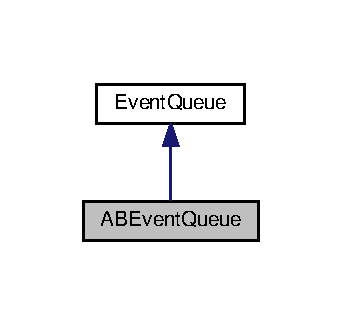
\includegraphics[width=164pt]{class_a_b_event_queue__inherit__graph}
\end{center}
\end{figure}


Collaboration diagram for A\+B\+Event\+Queue\+:
\nopagebreak
\begin{figure}[H]
\begin{center}
\leavevmode
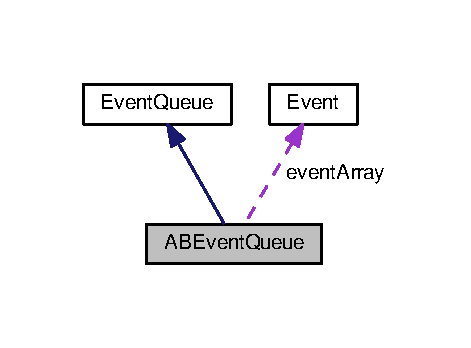
\includegraphics[width=226pt]{class_a_b_event_queue__coll__graph}
\end{center}
\end{figure}
\subsection*{Public Member Functions}
\begin{DoxyCompactItemize}
\item 
\hyperlink{class_a_b_event_queue_a8e2c4bb3d9315eb6fe227250d0d67cd7}{A\+B\+Event\+Queue} (int capacity)
\begin{DoxyCompactList}\small\item\em Constructs an empty queue with given capacity. \end{DoxyCompactList}\item 
\hyperlink{class_a_b_event_queue_a260b9f55c3ee4d3eae601e03ceb168ea}{A\+B\+Event\+Queue} (int capacity, int lob\+Arrival, int hib\+Arrival, int lob\+Duration, int hib\+Duration)
\begin{DoxyCompactList}\small\item\em Constructs a queue with given capacity and fills it randomly. \end{DoxyCompactList}\item 
\hyperlink{class_a_b_event_queue_a1294c9f60862ba7c384aee7291f82241}{$\sim$\+A\+B\+Event\+Queue} ()
\item 
int \hyperlink{class_a_b_event_queue_a59443fdc10016ddc1a6949f10c49c2ed}{length} ()
\item 
void \hyperlink{class_a_b_event_queue_adc34af0cd37c4ba62988eb2ee892357e}{add\+Back} (\hyperlink{struct_event}{Event} new\+Ev)
\item 
\hyperlink{struct_event}{Event} \hyperlink{class_a_b_event_queue_a0c1f23891bc06650703034f1854989d1}{pop\+Front} ()
\item 
\hyperlink{struct_event}{Event} \hyperlink{class_a_b_event_queue_aad5e909e29cb0eb71fbb5bf330e699eb}{peek\+Front} ()
\end{DoxyCompactItemize}
\subsection*{Private Attributes}
\begin{DoxyCompactItemize}
\item 
\hyperlink{struct_event}{Event} $\ast$ \hyperlink{class_a_b_event_queue_acb0bc62d6a21b4633ba50ae83fd4d79e}{event\+Array}
\item 
int \hyperlink{class_a_b_event_queue_a3f8d4bf9c3dad9b88a9f99220b567ed6}{cap}
\item 
int \hyperlink{class_a_b_event_queue_a26f1044edfb22cd3438b6da3839f6087}{len}
\end{DoxyCompactItemize}


\subsection{Detailed Description}
An Array-\/\+Based \hyperlink{struct_event}{Event} Queue. 

Capacity cannot change. 

\subsection{Constructor \& Destructor Documentation}
\index{A\+B\+Event\+Queue@{A\+B\+Event\+Queue}!A\+B\+Event\+Queue@{A\+B\+Event\+Queue}}
\index{A\+B\+Event\+Queue@{A\+B\+Event\+Queue}!A\+B\+Event\+Queue@{A\+B\+Event\+Queue}}
\subsubsection[{\texorpdfstring{A\+B\+Event\+Queue(int capacity)}{ABEventQueue(int capacity)}}]{\setlength{\rightskip}{0pt plus 5cm}A\+B\+Event\+Queue\+::\+A\+B\+Event\+Queue (
\begin{DoxyParamCaption}
\item[{int}]{capacity}
\end{DoxyParamCaption}
)}\hypertarget{class_a_b_event_queue_a8e2c4bb3d9315eb6fe227250d0d67cd7}{}\label{class_a_b_event_queue_a8e2c4bb3d9315eb6fe227250d0d67cd7}


Constructs an empty queue with given capacity. 


\begin{DoxyParams}{Parameters}
{\em capacity} & The capacity of the queue. \\
\hline
\end{DoxyParams}
\index{A\+B\+Event\+Queue@{A\+B\+Event\+Queue}!A\+B\+Event\+Queue@{A\+B\+Event\+Queue}}
\index{A\+B\+Event\+Queue@{A\+B\+Event\+Queue}!A\+B\+Event\+Queue@{A\+B\+Event\+Queue}}
\subsubsection[{\texorpdfstring{A\+B\+Event\+Queue(int capacity, int lob\+Arrival, int hib\+Arrival, int lob\+Duration, int hib\+Duration)}{ABEventQueue(int capacity, int lobArrival, int hibArrival, int lobDuration, int hibDuration)}}]{\setlength{\rightskip}{0pt plus 5cm}A\+B\+Event\+Queue\+::\+A\+B\+Event\+Queue (
\begin{DoxyParamCaption}
\item[{int}]{capacity, }
\item[{int}]{lob\+Arrival, }
\item[{int}]{hib\+Arrival, }
\item[{int}]{lob\+Duration, }
\item[{int}]{hib\+Duration}
\end{DoxyParamCaption}
)}\hypertarget{class_a_b_event_queue_a260b9f55c3ee4d3eae601e03ceb168ea}{}\label{class_a_b_event_queue_a260b9f55c3ee4d3eae601e03ceb168ea}


Constructs a queue with given capacity and fills it randomly. 


\begin{DoxyParams}{Parameters}
{\em capacity} & The capacity of the queue. \\
\hline
{\em lob\+Arrival} & Passed to fill\+Randomly. \\
\hline
{\em hib\+Arrival} & Passed to fill\+Randomly. \\
\hline
{\em lob\+Duration} & Passed to fill\+Randomly. \\
\hline
{\em hib\+Duration} & Passed to fill\+Randomly. \\
\hline
\end{DoxyParams}
\index{A\+B\+Event\+Queue@{A\+B\+Event\+Queue}!````~A\+B\+Event\+Queue@{$\sim$\+A\+B\+Event\+Queue}}
\index{````~A\+B\+Event\+Queue@{$\sim$\+A\+B\+Event\+Queue}!A\+B\+Event\+Queue@{A\+B\+Event\+Queue}}
\subsubsection[{\texorpdfstring{$\sim$\+A\+B\+Event\+Queue()}{~ABEventQueue()}}]{\setlength{\rightskip}{0pt plus 5cm}A\+B\+Event\+Queue\+::$\sim$\+A\+B\+Event\+Queue (
\begin{DoxyParamCaption}
{}
\end{DoxyParamCaption}
)}\hypertarget{class_a_b_event_queue_a1294c9f60862ba7c384aee7291f82241}{}\label{class_a_b_event_queue_a1294c9f60862ba7c384aee7291f82241}
Cleans up the queue. 

\subsection{Member Function Documentation}
\index{A\+B\+Event\+Queue@{A\+B\+Event\+Queue}!add\+Back@{add\+Back}}
\index{add\+Back@{add\+Back}!A\+B\+Event\+Queue@{A\+B\+Event\+Queue}}
\subsubsection[{\texorpdfstring{add\+Back(\+Event new\+Ev)}{addBack(Event newEv)}}]{\setlength{\rightskip}{0pt plus 5cm}void A\+B\+Event\+Queue\+::add\+Back (
\begin{DoxyParamCaption}
\item[{{\bf Event}}]{new\+Ev}
\end{DoxyParamCaption}
)\hspace{0.3cm}{\ttfamily [virtual]}}\hypertarget{class_a_b_event_queue_adc34af0cd37c4ba62988eb2ee892357e}{}\label{class_a_b_event_queue_adc34af0cd37c4ba62988eb2ee892357e}
Adds to the back of the queue. 

Implements \hyperlink{class_event_queue_ada350083afd0db585c0e023336e57d7b}{Event\+Queue}.

\index{A\+B\+Event\+Queue@{A\+B\+Event\+Queue}!length@{length}}
\index{length@{length}!A\+B\+Event\+Queue@{A\+B\+Event\+Queue}}
\subsubsection[{\texorpdfstring{length()}{length()}}]{\setlength{\rightskip}{0pt plus 5cm}int A\+B\+Event\+Queue\+::length (
\begin{DoxyParamCaption}
{}
\end{DoxyParamCaption}
)\hspace{0.3cm}{\ttfamily [virtual]}}\hypertarget{class_a_b_event_queue_a59443fdc10016ddc1a6949f10c49c2ed}{}\label{class_a_b_event_queue_a59443fdc10016ddc1a6949f10c49c2ed}
Get the length of the queue. 

Implements \hyperlink{class_event_queue_afc947be4a7122a4dd9a7ede8a7048f5c}{Event\+Queue}.

\index{A\+B\+Event\+Queue@{A\+B\+Event\+Queue}!peek\+Front@{peek\+Front}}
\index{peek\+Front@{peek\+Front}!A\+B\+Event\+Queue@{A\+B\+Event\+Queue}}
\subsubsection[{\texorpdfstring{peek\+Front()}{peekFront()}}]{\setlength{\rightskip}{0pt plus 5cm}{\bf Event} A\+B\+Event\+Queue\+::peek\+Front (
\begin{DoxyParamCaption}
{}
\end{DoxyParamCaption}
)\hspace{0.3cm}{\ttfamily [virtual]}}\hypertarget{class_a_b_event_queue_aad5e909e29cb0eb71fbb5bf330e699eb}{}\label{class_a_b_event_queue_aad5e909e29cb0eb71fbb5bf330e699eb}
Peek at the front of the queue. 

Implements \hyperlink{class_event_queue_ab16064eee197687eca21cedde00ab2ac}{Event\+Queue}.

\index{A\+B\+Event\+Queue@{A\+B\+Event\+Queue}!pop\+Front@{pop\+Front}}
\index{pop\+Front@{pop\+Front}!A\+B\+Event\+Queue@{A\+B\+Event\+Queue}}
\subsubsection[{\texorpdfstring{pop\+Front()}{popFront()}}]{\setlength{\rightskip}{0pt plus 5cm}{\bf Event} A\+B\+Event\+Queue\+::pop\+Front (
\begin{DoxyParamCaption}
{}
\end{DoxyParamCaption}
)\hspace{0.3cm}{\ttfamily [virtual]}}\hypertarget{class_a_b_event_queue_a0c1f23891bc06650703034f1854989d1}{}\label{class_a_b_event_queue_a0c1f23891bc06650703034f1854989d1}
Get and remove the event at the front of the queue. 

Implements \hyperlink{class_event_queue_a4f49434cc8ca60030f2b5737399527e2}{Event\+Queue}.



\subsection{Member Data Documentation}
\index{A\+B\+Event\+Queue@{A\+B\+Event\+Queue}!cap@{cap}}
\index{cap@{cap}!A\+B\+Event\+Queue@{A\+B\+Event\+Queue}}
\subsubsection[{\texorpdfstring{cap}{cap}}]{\setlength{\rightskip}{0pt plus 5cm}int A\+B\+Event\+Queue\+::cap\hspace{0.3cm}{\ttfamily [private]}}\hypertarget{class_a_b_event_queue_a3f8d4bf9c3dad9b88a9f99220b567ed6}{}\label{class_a_b_event_queue_a3f8d4bf9c3dad9b88a9f99220b567ed6}
\index{A\+B\+Event\+Queue@{A\+B\+Event\+Queue}!event\+Array@{event\+Array}}
\index{event\+Array@{event\+Array}!A\+B\+Event\+Queue@{A\+B\+Event\+Queue}}
\subsubsection[{\texorpdfstring{event\+Array}{eventArray}}]{\setlength{\rightskip}{0pt plus 5cm}{\bf Event}$\ast$ A\+B\+Event\+Queue\+::event\+Array\hspace{0.3cm}{\ttfamily [private]}}\hypertarget{class_a_b_event_queue_acb0bc62d6a21b4633ba50ae83fd4d79e}{}\label{class_a_b_event_queue_acb0bc62d6a21b4633ba50ae83fd4d79e}
\index{A\+B\+Event\+Queue@{A\+B\+Event\+Queue}!len@{len}}
\index{len@{len}!A\+B\+Event\+Queue@{A\+B\+Event\+Queue}}
\subsubsection[{\texorpdfstring{len}{len}}]{\setlength{\rightskip}{0pt plus 5cm}int A\+B\+Event\+Queue\+::len\hspace{0.3cm}{\ttfamily [private]}}\hypertarget{class_a_b_event_queue_a26f1044edfb22cd3438b6da3839f6087}{}\label{class_a_b_event_queue_a26f1044edfb22cd3438b6da3839f6087}


The documentation for this class was generated from the following files\+:\begin{DoxyCompactItemize}
\item 
\hyperlink{_a_b_event_queue_8h}{A\+B\+Event\+Queue.\+h}\item 
\hyperlink{_a_b_event_queue_8cpp}{A\+B\+Event\+Queue.\+cpp}\end{DoxyCompactItemize}

\hypertarget{struct_event}{}\section{Event Struct Reference}
\label{struct_event}\index{Event@{Event}}


{\ttfamily \#include $<$Event.\+h$>$}

\subsection*{Public Attributes}
\begin{DoxyCompactItemize}
\item 
int \hyperlink{struct_event_a3782e35ec08a4b5a8112b03404133be8}{arrival}
\item 
int \hyperlink{struct_event_aa083855a26c42d10c9dd5978f7066db8}{duration}
\end{DoxyCompactItemize}


\subsection{Member Data Documentation}
\index{Event@{Event}!arrival@{arrival}}
\index{arrival@{arrival}!Event@{Event}}
\subsubsection[{\texorpdfstring{arrival}{arrival}}]{\setlength{\rightskip}{0pt plus 5cm}int Event\+::arrival}\hypertarget{struct_event_a3782e35ec08a4b5a8112b03404133be8}{}\label{struct_event_a3782e35ec08a4b5a8112b03404133be8}
\index{Event@{Event}!duration@{duration}}
\index{duration@{duration}!Event@{Event}}
\subsubsection[{\texorpdfstring{duration}{duration}}]{\setlength{\rightskip}{0pt plus 5cm}int Event\+::duration}\hypertarget{struct_event_aa083855a26c42d10c9dd5978f7066db8}{}\label{struct_event_aa083855a26c42d10c9dd5978f7066db8}


The documentation for this struct was generated from the following file\+:\begin{DoxyCompactItemize}
\item 
\hyperlink{_event_8h}{Event.\+h}\end{DoxyCompactItemize}

\hypertarget{class_event_queue}{}\section{Event\+Queue Class Reference}
\label{class_event_queue}\index{Event\+Queue@{Event\+Queue}}


{\ttfamily \#include $<$Event\+Queue.\+h$>$}



Inheritance diagram for Event\+Queue\+:
\nopagebreak
\begin{figure}[H]
\begin{center}
\leavevmode
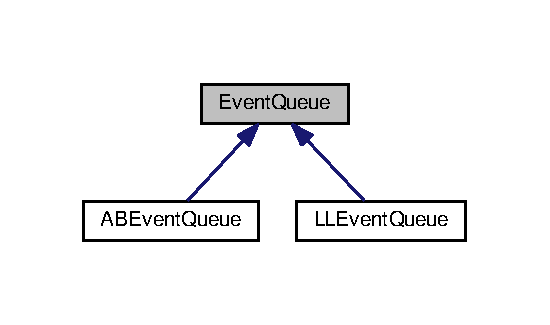
\includegraphics[width=264pt]{class_event_queue__inherit__graph}
\end{center}
\end{figure}
\subsection*{Public Member Functions}
\begin{DoxyCompactItemize}
\item 
virtual \hyperlink{class_event_queue_ac57db8e2366f2c6c594e6afc975e3b59}{$\sim$\+Event\+Queue} ()
\begin{DoxyCompactList}\small\item\em Cleans up the queue. \end{DoxyCompactList}\item 
virtual int \hyperlink{class_event_queue_afc947be4a7122a4dd9a7ede8a7048f5c}{length} ()=0
\begin{DoxyCompactList}\small\item\em Get the length of the queue. \end{DoxyCompactList}\item 
bool \hyperlink{class_event_queue_aa29d017edc0198d2113018d71d19369c}{is\+Empty} ()
\begin{DoxyCompactList}\small\item\em Get whether the queue is empty. \end{DoxyCompactList}\item 
void \hyperlink{class_event_queue_ad74cde47893e33c1288344f308c394d0}{fill\+Randomly} (int num, int lob\+Arrival, int hib\+Arrival, int lob\+Duration, int hib\+Duration)
\begin{DoxyCompactList}\small\item\em Fills the queue with randomly generated events. \end{DoxyCompactList}\item 
virtual void \hyperlink{class_event_queue_ada350083afd0db585c0e023336e57d7b}{add\+Back} (\hyperlink{struct_event}{Event} new\+Ev)=0
\begin{DoxyCompactList}\small\item\em Adds to the back of the queue. \end{DoxyCompactList}\item 
virtual \hyperlink{struct_event}{Event} \hyperlink{class_event_queue_a4f49434cc8ca60030f2b5737399527e2}{pop\+Front} ()=0
\begin{DoxyCompactList}\small\item\em Get and remove the event at the front of the queue. \end{DoxyCompactList}\item 
virtual \hyperlink{struct_event}{Event} \hyperlink{class_event_queue_ab16064eee197687eca21cedde00ab2ac}{peek\+Front} ()=0
\begin{DoxyCompactList}\small\item\em Peek at the front of the queue. \end{DoxyCompactList}\end{DoxyCompactItemize}


\subsection{Constructor \& Destructor Documentation}
\index{Event\+Queue@{Event\+Queue}!````~Event\+Queue@{$\sim$\+Event\+Queue}}
\index{````~Event\+Queue@{$\sim$\+Event\+Queue}!Event\+Queue@{Event\+Queue}}
\subsubsection[{\texorpdfstring{$\sim$\+Event\+Queue()}{~EventQueue()}}]{\setlength{\rightskip}{0pt plus 5cm}Event\+Queue\+::$\sim$\+Event\+Queue (
\begin{DoxyParamCaption}
{}
\end{DoxyParamCaption}
)\hspace{0.3cm}{\ttfamily [virtual]}}\hypertarget{class_event_queue_ac57db8e2366f2c6c594e6afc975e3b59}{}\label{class_event_queue_ac57db8e2366f2c6c594e6afc975e3b59}


Cleans up the queue. 



\subsection{Member Function Documentation}
\index{Event\+Queue@{Event\+Queue}!add\+Back@{add\+Back}}
\index{add\+Back@{add\+Back}!Event\+Queue@{Event\+Queue}}
\subsubsection[{\texorpdfstring{add\+Back(\+Event new\+Ev)=0}{addBack(Event newEv)=0}}]{\setlength{\rightskip}{0pt plus 5cm}virtual void Event\+Queue\+::add\+Back (
\begin{DoxyParamCaption}
\item[{{\bf Event}}]{new\+Ev}
\end{DoxyParamCaption}
)\hspace{0.3cm}{\ttfamily [pure virtual]}}\hypertarget{class_event_queue_ada350083afd0db585c0e023336e57d7b}{}\label{class_event_queue_ada350083afd0db585c0e023336e57d7b}


Adds to the back of the queue. 


\begin{DoxyParams}{Parameters}
{\em new\+Ev} & The event to add. \\
\hline
\end{DoxyParams}


Implemented in \hyperlink{class_l_l_event_queue_a0965f4171186e119b2e63c1fbdafedd8}{L\+L\+Event\+Queue}, and \hyperlink{class_a_b_event_queue_adc34af0cd37c4ba62988eb2ee892357e}{A\+B\+Event\+Queue}.

\index{Event\+Queue@{Event\+Queue}!fill\+Randomly@{fill\+Randomly}}
\index{fill\+Randomly@{fill\+Randomly}!Event\+Queue@{Event\+Queue}}
\subsubsection[{\texorpdfstring{fill\+Randomly(int num, int lob\+Arrival, int hib\+Arrival, int lob\+Duration, int hib\+Duration)}{fillRandomly(int num, int lobArrival, int hibArrival, int lobDuration, int hibDuration)}}]{\setlength{\rightskip}{0pt plus 5cm}void Event\+Queue\+::fill\+Randomly (
\begin{DoxyParamCaption}
\item[{int}]{num, }
\item[{int}]{lob\+Arrival, }
\item[{int}]{hib\+Arrival, }
\item[{int}]{lob\+Duration, }
\item[{int}]{hib\+Duration}
\end{DoxyParamCaption}
)}\hypertarget{class_event_queue_ad74cde47893e33c1288344f308c394d0}{}\label{class_event_queue_ad74cde47893e33c1288344f308c394d0}


Fills the queue with randomly generated events. 

num The number of events to generate. 
\begin{DoxyParams}{Parameters}
{\em lob\+Arrival} & The low bound for arrival times. \\
\hline
{\em hib\+Arrival} & The high bound for arrival times. \\
\hline
{\em lob\+Duration} & The low bound for duration times. \\
\hline
{\em hib\+Duration} & The high bound for duration times. \\
\hline
\end{DoxyParams}
\index{Event\+Queue@{Event\+Queue}!is\+Empty@{is\+Empty}}
\index{is\+Empty@{is\+Empty}!Event\+Queue@{Event\+Queue}}
\subsubsection[{\texorpdfstring{is\+Empty()}{isEmpty()}}]{\setlength{\rightskip}{0pt plus 5cm}bool Event\+Queue\+::is\+Empty (
\begin{DoxyParamCaption}
{}
\end{DoxyParamCaption}
)}\hypertarget{class_event_queue_aa29d017edc0198d2113018d71d19369c}{}\label{class_event_queue_aa29d017edc0198d2113018d71d19369c}


Get whether the queue is empty. 

\begin{DoxyReturn}{Returns}
True if empty; false otherwise. 
\end{DoxyReturn}
\index{Event\+Queue@{Event\+Queue}!length@{length}}
\index{length@{length}!Event\+Queue@{Event\+Queue}}
\subsubsection[{\texorpdfstring{length()=0}{length()=0}}]{\setlength{\rightskip}{0pt plus 5cm}virtual int Event\+Queue\+::length (
\begin{DoxyParamCaption}
{}
\end{DoxyParamCaption}
)\hspace{0.3cm}{\ttfamily [pure virtual]}}\hypertarget{class_event_queue_afc947be4a7122a4dd9a7ede8a7048f5c}{}\label{class_event_queue_afc947be4a7122a4dd9a7ede8a7048f5c}


Get the length of the queue. 

\begin{DoxyReturn}{Returns}
The length of the queue. 
\end{DoxyReturn}


Implemented in \hyperlink{class_l_l_event_queue_a6ca56aeb714d44bb3c93748c4fe87bb6}{L\+L\+Event\+Queue}, and \hyperlink{class_a_b_event_queue_a59443fdc10016ddc1a6949f10c49c2ed}{A\+B\+Event\+Queue}.

\index{Event\+Queue@{Event\+Queue}!peek\+Front@{peek\+Front}}
\index{peek\+Front@{peek\+Front}!Event\+Queue@{Event\+Queue}}
\subsubsection[{\texorpdfstring{peek\+Front()=0}{peekFront()=0}}]{\setlength{\rightskip}{0pt plus 5cm}virtual {\bf Event} Event\+Queue\+::peek\+Front (
\begin{DoxyParamCaption}
{}
\end{DoxyParamCaption}
)\hspace{0.3cm}{\ttfamily [pure virtual]}}\hypertarget{class_event_queue_ab16064eee197687eca21cedde00ab2ac}{}\label{class_event_queue_ab16064eee197687eca21cedde00ab2ac}


Peek at the front of the queue. 

\begin{DoxyReturn}{Returns}
The event at the front of the queue. 
\end{DoxyReturn}


Implemented in \hyperlink{class_l_l_event_queue_a363c623da23cfc4baa0ff29c1801759f}{L\+L\+Event\+Queue}, and \hyperlink{class_a_b_event_queue_aad5e909e29cb0eb71fbb5bf330e699eb}{A\+B\+Event\+Queue}.

\index{Event\+Queue@{Event\+Queue}!pop\+Front@{pop\+Front}}
\index{pop\+Front@{pop\+Front}!Event\+Queue@{Event\+Queue}}
\subsubsection[{\texorpdfstring{pop\+Front()=0}{popFront()=0}}]{\setlength{\rightskip}{0pt plus 5cm}virtual {\bf Event} Event\+Queue\+::pop\+Front (
\begin{DoxyParamCaption}
{}
\end{DoxyParamCaption}
)\hspace{0.3cm}{\ttfamily [pure virtual]}}\hypertarget{class_event_queue_a4f49434cc8ca60030f2b5737399527e2}{}\label{class_event_queue_a4f49434cc8ca60030f2b5737399527e2}


Get and remove the event at the front of the queue. 

\begin{DoxyReturn}{Returns}
The event at the front of the queue. 
\end{DoxyReturn}


Implemented in \hyperlink{class_l_l_event_queue_aad3c57796c1ba1e06933083d714722e7}{L\+L\+Event\+Queue}, and \hyperlink{class_a_b_event_queue_a0c1f23891bc06650703034f1854989d1}{A\+B\+Event\+Queue}.



The documentation for this class was generated from the following files\+:\begin{DoxyCompactItemize}
\item 
\hyperlink{_event_queue_8h}{Event\+Queue.\+h}\item 
\hyperlink{_event_queue_8cpp}{Event\+Queue.\+cpp}\end{DoxyCompactItemize}

\hypertarget{struct_l_l_e_q_node}{}\section{L\+L\+E\+Q\+Node Struct Reference}
\label{struct_l_l_e_q_node}\index{L\+L\+E\+Q\+Node@{L\+L\+E\+Q\+Node}}


A node in an \hyperlink{class_l_l_event_queue}{L\+L\+Event\+Queue}.  




{\ttfamily \#include $<$L\+L\+Event\+Queue.\+h$>$}



Collaboration diagram for L\+L\+E\+Q\+Node\+:
\nopagebreak
\begin{figure}[H]
\begin{center}
\leavevmode
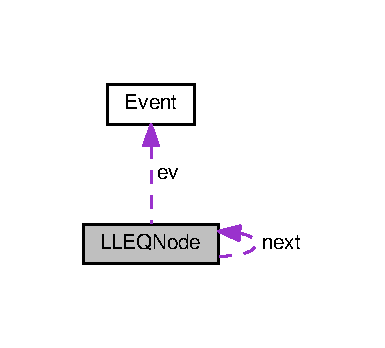
\includegraphics[width=185pt]{struct_l_l_e_q_node__coll__graph}
\end{center}
\end{figure}
\subsection*{Public Attributes}
\begin{DoxyCompactItemize}
\item 
\hyperlink{struct_event}{Event} \hyperlink{struct_l_l_e_q_node_a93737f2108ade25891fbbc3359a62e32}{ev}
\item 
\hyperlink{struct_l_l_e_q_node}{L\+L\+E\+Q\+Node} $\ast$ \hyperlink{struct_l_l_e_q_node_a7c95e7d5f2e3d03def48228b509212f6}{next}
\end{DoxyCompactItemize}


\subsection{Detailed Description}
A node in an \hyperlink{class_l_l_event_queue}{L\+L\+Event\+Queue}. 

\subsection{Member Data Documentation}
\index{L\+L\+E\+Q\+Node@{L\+L\+E\+Q\+Node}!ev@{ev}}
\index{ev@{ev}!L\+L\+E\+Q\+Node@{L\+L\+E\+Q\+Node}}
\subsubsection[{\texorpdfstring{ev}{ev}}]{\setlength{\rightskip}{0pt plus 5cm}{\bf Event} L\+L\+E\+Q\+Node\+::ev}\hypertarget{struct_l_l_e_q_node_a93737f2108ade25891fbbc3359a62e32}{}\label{struct_l_l_e_q_node_a93737f2108ade25891fbbc3359a62e32}
\index{L\+L\+E\+Q\+Node@{L\+L\+E\+Q\+Node}!next@{next}}
\index{next@{next}!L\+L\+E\+Q\+Node@{L\+L\+E\+Q\+Node}}
\subsubsection[{\texorpdfstring{next}{next}}]{\setlength{\rightskip}{0pt plus 5cm}{\bf L\+L\+E\+Q\+Node}$\ast$ L\+L\+E\+Q\+Node\+::next}\hypertarget{struct_l_l_e_q_node_a7c95e7d5f2e3d03def48228b509212f6}{}\label{struct_l_l_e_q_node_a7c95e7d5f2e3d03def48228b509212f6}


The documentation for this struct was generated from the following file\+:\begin{DoxyCompactItemize}
\item 
\hyperlink{_l_l_event_queue_8h}{L\+L\+Event\+Queue.\+h}\end{DoxyCompactItemize}

\hypertarget{class_l_l_event_queue}{}\section{L\+L\+Event\+Queue Class Reference}
\label{class_l_l_event_queue}\index{L\+L\+Event\+Queue@{L\+L\+Event\+Queue}}


A Linked-\/\+List-\/\+Based \hyperlink{struct_event}{Event} Queue.  




{\ttfamily \#include $<$L\+L\+Event\+Queue.\+h$>$}



Inheritance diagram for L\+L\+Event\+Queue\+:
\nopagebreak
\begin{figure}[H]
\begin{center}
\leavevmode
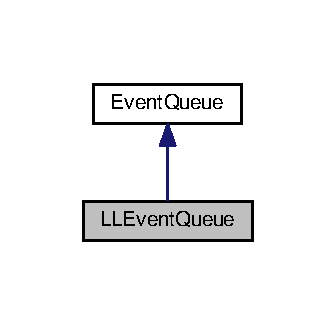
\includegraphics[width=161pt]{class_l_l_event_queue__inherit__graph}
\end{center}
\end{figure}


Collaboration diagram for L\+L\+Event\+Queue\+:
\nopagebreak
\begin{figure}[H]
\begin{center}
\leavevmode
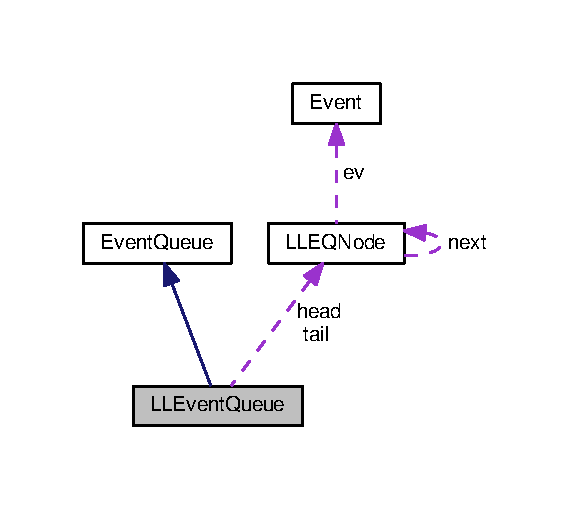
\includegraphics[width=274pt]{class_l_l_event_queue__coll__graph}
\end{center}
\end{figure}
\subsection*{Public Member Functions}
\begin{DoxyCompactItemize}
\item 
\hyperlink{class_l_l_event_queue_ab778c3122c7ac7ebfd0de6e1d469efad}{L\+L\+Event\+Queue} ()
\begin{DoxyCompactList}\small\item\em Constructs an empty queue. \end{DoxyCompactList}\item 
\hyperlink{class_l_l_event_queue_ac3a67029f7d9a85b6ec3a3daadf58bd3}{L\+L\+Event\+Queue} (int num, int lob\+Arrival, int hib\+Arrival, int lob\+Duration, int hib\+Duration)
\begin{DoxyCompactList}\small\item\em Constructs a queue and fills it randomly. \end{DoxyCompactList}\item 
\hyperlink{class_l_l_event_queue_a5bdaa10284e0fb6f3a51fc09ce6e2322}{$\sim$\+L\+L\+Event\+Queue} ()
\item 
int \hyperlink{class_l_l_event_queue_a6ca56aeb714d44bb3c93748c4fe87bb6}{length} ()
\item 
void \hyperlink{class_l_l_event_queue_a0965f4171186e119b2e63c1fbdafedd8}{add\+Back} (\hyperlink{struct_event}{Event} new\+Ev)
\item 
\hyperlink{struct_event}{Event} \hyperlink{class_l_l_event_queue_aad3c57796c1ba1e06933083d714722e7}{pop\+Front} ()
\item 
\hyperlink{struct_event}{Event} \hyperlink{class_l_l_event_queue_a363c623da23cfc4baa0ff29c1801759f}{peek\+Front} ()
\end{DoxyCompactItemize}
\subsection*{Public Attributes}
\begin{DoxyCompactItemize}
\item 
\hyperlink{struct_l_l_e_q_node}{L\+L\+E\+Q\+Node} $\ast$ \hyperlink{class_l_l_event_queue_a9f789093fd1f9af546885d589ccf3271}{head}
\item 
\hyperlink{struct_l_l_e_q_node}{L\+L\+E\+Q\+Node} $\ast$ \hyperlink{class_l_l_event_queue_a1f5ddd89f1a0b4c7e475b364b0084564}{tail}
\item 
int \hyperlink{class_l_l_event_queue_a86b7dfcff49beb1443b57d0610725c3b}{len}
\end{DoxyCompactItemize}


\subsection{Detailed Description}
A Linked-\/\+List-\/\+Based \hyperlink{struct_event}{Event} Queue. 

\subsection{Constructor \& Destructor Documentation}
\index{L\+L\+Event\+Queue@{L\+L\+Event\+Queue}!L\+L\+Event\+Queue@{L\+L\+Event\+Queue}}
\index{L\+L\+Event\+Queue@{L\+L\+Event\+Queue}!L\+L\+Event\+Queue@{L\+L\+Event\+Queue}}
\subsubsection[{\texorpdfstring{L\+L\+Event\+Queue()}{LLEventQueue()}}]{\setlength{\rightskip}{0pt plus 5cm}L\+L\+Event\+Queue\+::\+L\+L\+Event\+Queue (
\begin{DoxyParamCaption}
{}
\end{DoxyParamCaption}
)}\hypertarget{class_l_l_event_queue_ab778c3122c7ac7ebfd0de6e1d469efad}{}\label{class_l_l_event_queue_ab778c3122c7ac7ebfd0de6e1d469efad}


Constructs an empty queue. 

\index{L\+L\+Event\+Queue@{L\+L\+Event\+Queue}!L\+L\+Event\+Queue@{L\+L\+Event\+Queue}}
\index{L\+L\+Event\+Queue@{L\+L\+Event\+Queue}!L\+L\+Event\+Queue@{L\+L\+Event\+Queue}}
\subsubsection[{\texorpdfstring{L\+L\+Event\+Queue(int num, int lob\+Arrival, int hib\+Arrival, int lob\+Duration, int hib\+Duration)}{LLEventQueue(int num, int lobArrival, int hibArrival, int lobDuration, int hibDuration)}}]{\setlength{\rightskip}{0pt plus 5cm}L\+L\+Event\+Queue\+::\+L\+L\+Event\+Queue (
\begin{DoxyParamCaption}
\item[{int}]{num, }
\item[{int}]{lob\+Arrival, }
\item[{int}]{hib\+Arrival, }
\item[{int}]{lob\+Duration, }
\item[{int}]{hib\+Duration}
\end{DoxyParamCaption}
)}\hypertarget{class_l_l_event_queue_ac3a67029f7d9a85b6ec3a3daadf58bd3}{}\label{class_l_l_event_queue_ac3a67029f7d9a85b6ec3a3daadf58bd3}


Constructs a queue and fills it randomly. 


\begin{DoxyParams}{Parameters}
{\em num} & Passed to fill\+Randomly. \\
\hline
{\em lob\+Arrival} & Passed to fill\+Randomly. \\
\hline
{\em hib\+Arrival} & Passed to fill\+Randomly. \\
\hline
{\em lob\+Duration} & Passed to fill\+Randomly. \\
\hline
{\em hib\+Duration} & Passed to fill\+Randomly. \\
\hline
\end{DoxyParams}
\index{L\+L\+Event\+Queue@{L\+L\+Event\+Queue}!````~L\+L\+Event\+Queue@{$\sim$\+L\+L\+Event\+Queue}}
\index{````~L\+L\+Event\+Queue@{$\sim$\+L\+L\+Event\+Queue}!L\+L\+Event\+Queue@{L\+L\+Event\+Queue}}
\subsubsection[{\texorpdfstring{$\sim$\+L\+L\+Event\+Queue()}{~LLEventQueue()}}]{\setlength{\rightskip}{0pt plus 5cm}L\+L\+Event\+Queue\+::$\sim$\+L\+L\+Event\+Queue (
\begin{DoxyParamCaption}
{}
\end{DoxyParamCaption}
)}\hypertarget{class_l_l_event_queue_a5bdaa10284e0fb6f3a51fc09ce6e2322}{}\label{class_l_l_event_queue_a5bdaa10284e0fb6f3a51fc09ce6e2322}
Cleans up the queue. 

\subsection{Member Function Documentation}
\index{L\+L\+Event\+Queue@{L\+L\+Event\+Queue}!add\+Back@{add\+Back}}
\index{add\+Back@{add\+Back}!L\+L\+Event\+Queue@{L\+L\+Event\+Queue}}
\subsubsection[{\texorpdfstring{add\+Back(\+Event new\+Ev)}{addBack(Event newEv)}}]{\setlength{\rightskip}{0pt plus 5cm}void L\+L\+Event\+Queue\+::add\+Back (
\begin{DoxyParamCaption}
\item[{{\bf Event}}]{new\+Ev}
\end{DoxyParamCaption}
)\hspace{0.3cm}{\ttfamily [virtual]}}\hypertarget{class_l_l_event_queue_a0965f4171186e119b2e63c1fbdafedd8}{}\label{class_l_l_event_queue_a0965f4171186e119b2e63c1fbdafedd8}
Adds to the back of the queue. 

Implements \hyperlink{class_event_queue_ada350083afd0db585c0e023336e57d7b}{Event\+Queue}.

\index{L\+L\+Event\+Queue@{L\+L\+Event\+Queue}!length@{length}}
\index{length@{length}!L\+L\+Event\+Queue@{L\+L\+Event\+Queue}}
\subsubsection[{\texorpdfstring{length()}{length()}}]{\setlength{\rightskip}{0pt plus 5cm}int L\+L\+Event\+Queue\+::length (
\begin{DoxyParamCaption}
{}
\end{DoxyParamCaption}
)\hspace{0.3cm}{\ttfamily [virtual]}}\hypertarget{class_l_l_event_queue_a6ca56aeb714d44bb3c93748c4fe87bb6}{}\label{class_l_l_event_queue_a6ca56aeb714d44bb3c93748c4fe87bb6}
Get the length of the queue. 

Implements \hyperlink{class_event_queue_afc947be4a7122a4dd9a7ede8a7048f5c}{Event\+Queue}.

\index{L\+L\+Event\+Queue@{L\+L\+Event\+Queue}!peek\+Front@{peek\+Front}}
\index{peek\+Front@{peek\+Front}!L\+L\+Event\+Queue@{L\+L\+Event\+Queue}}
\subsubsection[{\texorpdfstring{peek\+Front()}{peekFront()}}]{\setlength{\rightskip}{0pt plus 5cm}{\bf Event} L\+L\+Event\+Queue\+::peek\+Front (
\begin{DoxyParamCaption}
{}
\end{DoxyParamCaption}
)\hspace{0.3cm}{\ttfamily [virtual]}}\hypertarget{class_l_l_event_queue_a363c623da23cfc4baa0ff29c1801759f}{}\label{class_l_l_event_queue_a363c623da23cfc4baa0ff29c1801759f}
Peek at the front of the queue. 

Implements \hyperlink{class_event_queue_ab16064eee197687eca21cedde00ab2ac}{Event\+Queue}.

\index{L\+L\+Event\+Queue@{L\+L\+Event\+Queue}!pop\+Front@{pop\+Front}}
\index{pop\+Front@{pop\+Front}!L\+L\+Event\+Queue@{L\+L\+Event\+Queue}}
\subsubsection[{\texorpdfstring{pop\+Front()}{popFront()}}]{\setlength{\rightskip}{0pt plus 5cm}{\bf Event} L\+L\+Event\+Queue\+::pop\+Front (
\begin{DoxyParamCaption}
{}
\end{DoxyParamCaption}
)\hspace{0.3cm}{\ttfamily [virtual]}}\hypertarget{class_l_l_event_queue_aad3c57796c1ba1e06933083d714722e7}{}\label{class_l_l_event_queue_aad3c57796c1ba1e06933083d714722e7}
Get and remove the event at the front of the queue. 

Implements \hyperlink{class_event_queue_a4f49434cc8ca60030f2b5737399527e2}{Event\+Queue}.



\subsection{Member Data Documentation}
\index{L\+L\+Event\+Queue@{L\+L\+Event\+Queue}!head@{head}}
\index{head@{head}!L\+L\+Event\+Queue@{L\+L\+Event\+Queue}}
\subsubsection[{\texorpdfstring{head}{head}}]{\setlength{\rightskip}{0pt plus 5cm}{\bf L\+L\+E\+Q\+Node}$\ast$ L\+L\+Event\+Queue\+::head}\hypertarget{class_l_l_event_queue_a9f789093fd1f9af546885d589ccf3271}{}\label{class_l_l_event_queue_a9f789093fd1f9af546885d589ccf3271}
\index{L\+L\+Event\+Queue@{L\+L\+Event\+Queue}!len@{len}}
\index{len@{len}!L\+L\+Event\+Queue@{L\+L\+Event\+Queue}}
\subsubsection[{\texorpdfstring{len}{len}}]{\setlength{\rightskip}{0pt plus 5cm}int L\+L\+Event\+Queue\+::len}\hypertarget{class_l_l_event_queue_a86b7dfcff49beb1443b57d0610725c3b}{}\label{class_l_l_event_queue_a86b7dfcff49beb1443b57d0610725c3b}
\index{L\+L\+Event\+Queue@{L\+L\+Event\+Queue}!tail@{tail}}
\index{tail@{tail}!L\+L\+Event\+Queue@{L\+L\+Event\+Queue}}
\subsubsection[{\texorpdfstring{tail}{tail}}]{\setlength{\rightskip}{0pt plus 5cm}{\bf L\+L\+E\+Q\+Node}$\ast$ L\+L\+Event\+Queue\+::tail}\hypertarget{class_l_l_event_queue_a1f5ddd89f1a0b4c7e475b364b0084564}{}\label{class_l_l_event_queue_a1f5ddd89f1a0b4c7e475b364b0084564}


The documentation for this class was generated from the following files\+:\begin{DoxyCompactItemize}
\item 
\hyperlink{_l_l_event_queue_8h}{L\+L\+Event\+Queue.\+h}\item 
\hyperlink{_l_l_event_queue_8cpp}{L\+L\+Event\+Queue.\+cpp}\end{DoxyCompactItemize}

\hypertarget{class_teller}{}\section{Teller Class Reference}
\label{class_teller}\index{Teller@{Teller}}


Models a bank teller.  




{\ttfamily \#include $<$Teller\+Setup.\+h$>$}



Inheritance diagram for Teller\+:
\nopagebreak
\begin{figure}[H]
\begin{center}
\leavevmode
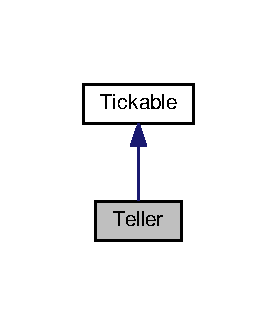
\includegraphics[width=133pt]{class_teller__inherit__graph}
\end{center}
\end{figure}


Collaboration diagram for Teller\+:
\nopagebreak
\begin{figure}[H]
\begin{center}
\leavevmode
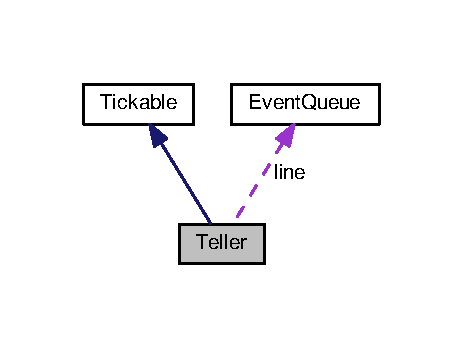
\includegraphics[width=222pt]{class_teller__coll__graph}
\end{center}
\end{figure}
\subsection*{Public Member Functions}
\begin{DoxyCompactItemize}
\item 
\hyperlink{class_teller_ad4e81dd3ee7aa9fec8464e97754a89f2}{Teller} (\hyperlink{class_event_queue}{Event\+Queue} $\ast$ln, int $\ast$nc, double $\ast$twt, double $\ast$mwt)
\begin{DoxyCompactList}\small\item\em Construct a \hyperlink{class_teller}{Teller} with given stat vars and source line. \end{DoxyCompactList}\item 
void \hyperlink{class_teller_aa8cf7bb201a88b959b42a3c4358565c3}{tick} (int now)
\item 
int \hyperlink{class_teller_a10106b3a286c21870bde1751aec0f9b6}{when\+Next} ()
\item 
void \hyperlink{class_teller_aaedc2bff64e9223f295cf9f05226b12e}{finish} (int now)
\begin{DoxyCompactList}\small\item\em Finishes the \hyperlink{class_teller}{Teller} model. Should be called at sim end. \end{DoxyCompactList}\end{DoxyCompactItemize}
\subsection*{Public Attributes}
\begin{DoxyCompactItemize}
\item 
int \hyperlink{class_teller_a09db98c5db957cd1937b3b5e9fa2820b}{idle\+Time}
\end{DoxyCompactItemize}
\subsection*{Protected Attributes}
\begin{DoxyCompactItemize}
\item 
\hyperlink{class_event_queue}{Event\+Queue} $\ast$ \hyperlink{class_teller_ad43bf4c0eeee493a6dce005ba95527a4}{line}
\item 
int $\ast$ \hyperlink{class_teller_aeb31b3f7b01ecc86be2aecf9899d29cd}{num\+Customers}
\item 
double $\ast$ \hyperlink{class_teller_a0fe70e6fab108e4f1f478835d0856b38}{tot\+Wait\+Time}
\item 
double $\ast$ \hyperlink{class_teller_af14fc15803a686d5a4a94e5538f15077}{max\+Wait\+Time}
\item 
int \hyperlink{class_teller_a7b9a77eab83010cba4e56ec487c90f9a}{idle\+Start}
\item 
bool \hyperlink{class_teller_a755cb7ba947e09ef875201bdaa38736e}{busy}
\item 
int \hyperlink{class_teller_a7ca8b1718a8dfcc84c300496430981af}{busy\+Until}
\end{DoxyCompactItemize}


\subsection{Detailed Description}
Models a bank teller. 

For use by \hyperlink{class_teller_setup}{Teller\+Setup}. 

\subsection{Constructor \& Destructor Documentation}
\index{Teller@{Teller}!Teller@{Teller}}
\index{Teller@{Teller}!Teller@{Teller}}
\subsubsection[{\texorpdfstring{Teller(\+Event\+Queue $\ast$ln, int $\ast$nc, double $\ast$twt, double $\ast$mwt)}{Teller(EventQueue *ln, int *nc, double *twt, double *mwt)}}]{\setlength{\rightskip}{0pt plus 5cm}Teller\+::\+Teller (
\begin{DoxyParamCaption}
\item[{{\bf Event\+Queue} $\ast$}]{ln, }
\item[{int $\ast$}]{nc, }
\item[{double $\ast$}]{twt, }
\item[{double $\ast$}]{mwt}
\end{DoxyParamCaption}
)}\hypertarget{class_teller_ad4e81dd3ee7aa9fec8464e97754a89f2}{}\label{class_teller_ad4e81dd3ee7aa9fec8464e97754a89f2}


Construct a \hyperlink{class_teller}{Teller} with given stat vars and source line. 


\begin{DoxyParams}{Parameters}
{\em ln} & The line to draw customers from. \\
\hline
{\em nc} & Pointer to the customer counter. \\
\hline
{\em twt} & Pointer to the wait time counter. \\
\hline
{\em mwt} & Pointer to the max wait time. \\
\hline
\end{DoxyParams}


\subsection{Member Function Documentation}
\index{Teller@{Teller}!finish@{finish}}
\index{finish@{finish}!Teller@{Teller}}
\subsubsection[{\texorpdfstring{finish(int now)}{finish(int now)}}]{\setlength{\rightskip}{0pt plus 5cm}void Teller\+::finish (
\begin{DoxyParamCaption}
\item[{int}]{now}
\end{DoxyParamCaption}
)}\hypertarget{class_teller_aaedc2bff64e9223f295cf9f05226b12e}{}\label{class_teller_aaedc2bff64e9223f295cf9f05226b12e}


Finishes the \hyperlink{class_teller}{Teller} model. Should be called at sim end. 


\begin{DoxyParams}{Parameters}
{\em now} & The last tick. \\
\hline
\end{DoxyParams}
\index{Teller@{Teller}!tick@{tick}}
\index{tick@{tick}!Teller@{Teller}}
\subsubsection[{\texorpdfstring{tick(int now)}{tick(int now)}}]{\setlength{\rightskip}{0pt plus 5cm}void Teller\+::tick (
\begin{DoxyParamCaption}
\item[{int}]{now}
\end{DoxyParamCaption}
)\hspace{0.3cm}{\ttfamily [virtual]}}\hypertarget{class_teller_aa8cf7bb201a88b959b42a3c4358565c3}{}\label{class_teller_aa8cf7bb201a88b959b42a3c4358565c3}
Do one tick at the given time. 

Implements \hyperlink{class_tickable_a0ca181a29c3e1539e4221d2cbcfa83c2}{Tickable}.

\index{Teller@{Teller}!when\+Next@{when\+Next}}
\index{when\+Next@{when\+Next}!Teller@{Teller}}
\subsubsection[{\texorpdfstring{when\+Next()}{whenNext()}}]{\setlength{\rightskip}{0pt plus 5cm}int Teller\+::when\+Next (
\begin{DoxyParamCaption}
{}
\end{DoxyParamCaption}
)\hspace{0.3cm}{\ttfamily [virtual]}}\hypertarget{class_teller_a10106b3a286c21870bde1751aec0f9b6}{}\label{class_teller_a10106b3a286c21870bde1751aec0f9b6}
Get when this tickable needs to be ticked next. 

Implements \hyperlink{class_tickable_ac65be54f32d39d1450a37cf4acb1ad15}{Tickable}.



\subsection{Member Data Documentation}
\index{Teller@{Teller}!busy@{busy}}
\index{busy@{busy}!Teller@{Teller}}
\subsubsection[{\texorpdfstring{busy}{busy}}]{\setlength{\rightskip}{0pt plus 5cm}bool Teller\+::busy\hspace{0.3cm}{\ttfamily [protected]}}\hypertarget{class_teller_a755cb7ba947e09ef875201bdaa38736e}{}\label{class_teller_a755cb7ba947e09ef875201bdaa38736e}
\index{Teller@{Teller}!busy\+Until@{busy\+Until}}
\index{busy\+Until@{busy\+Until}!Teller@{Teller}}
\subsubsection[{\texorpdfstring{busy\+Until}{busyUntil}}]{\setlength{\rightskip}{0pt plus 5cm}int Teller\+::busy\+Until\hspace{0.3cm}{\ttfamily [protected]}}\hypertarget{class_teller_a7ca8b1718a8dfcc84c300496430981af}{}\label{class_teller_a7ca8b1718a8dfcc84c300496430981af}
\index{Teller@{Teller}!idle\+Start@{idle\+Start}}
\index{idle\+Start@{idle\+Start}!Teller@{Teller}}
\subsubsection[{\texorpdfstring{idle\+Start}{idleStart}}]{\setlength{\rightskip}{0pt plus 5cm}int Teller\+::idle\+Start\hspace{0.3cm}{\ttfamily [protected]}}\hypertarget{class_teller_a7b9a77eab83010cba4e56ec487c90f9a}{}\label{class_teller_a7b9a77eab83010cba4e56ec487c90f9a}
\index{Teller@{Teller}!idle\+Time@{idle\+Time}}
\index{idle\+Time@{idle\+Time}!Teller@{Teller}}
\subsubsection[{\texorpdfstring{idle\+Time}{idleTime}}]{\setlength{\rightskip}{0pt plus 5cm}int Teller\+::idle\+Time}\hypertarget{class_teller_a09db98c5db957cd1937b3b5e9fa2820b}{}\label{class_teller_a09db98c5db957cd1937b3b5e9fa2820b}
\index{Teller@{Teller}!line@{line}}
\index{line@{line}!Teller@{Teller}}
\subsubsection[{\texorpdfstring{line}{line}}]{\setlength{\rightskip}{0pt plus 5cm}{\bf Event\+Queue}$\ast$ Teller\+::line\hspace{0.3cm}{\ttfamily [protected]}}\hypertarget{class_teller_ad43bf4c0eeee493a6dce005ba95527a4}{}\label{class_teller_ad43bf4c0eeee493a6dce005ba95527a4}
\index{Teller@{Teller}!max\+Wait\+Time@{max\+Wait\+Time}}
\index{max\+Wait\+Time@{max\+Wait\+Time}!Teller@{Teller}}
\subsubsection[{\texorpdfstring{max\+Wait\+Time}{maxWaitTime}}]{\setlength{\rightskip}{0pt plus 5cm}double$\ast$ Teller\+::max\+Wait\+Time\hspace{0.3cm}{\ttfamily [protected]}}\hypertarget{class_teller_af14fc15803a686d5a4a94e5538f15077}{}\label{class_teller_af14fc15803a686d5a4a94e5538f15077}
\index{Teller@{Teller}!num\+Customers@{num\+Customers}}
\index{num\+Customers@{num\+Customers}!Teller@{Teller}}
\subsubsection[{\texorpdfstring{num\+Customers}{numCustomers}}]{\setlength{\rightskip}{0pt plus 5cm}int$\ast$ Teller\+::num\+Customers\hspace{0.3cm}{\ttfamily [protected]}}\hypertarget{class_teller_aeb31b3f7b01ecc86be2aecf9899d29cd}{}\label{class_teller_aeb31b3f7b01ecc86be2aecf9899d29cd}
\index{Teller@{Teller}!tot\+Wait\+Time@{tot\+Wait\+Time}}
\index{tot\+Wait\+Time@{tot\+Wait\+Time}!Teller@{Teller}}
\subsubsection[{\texorpdfstring{tot\+Wait\+Time}{totWaitTime}}]{\setlength{\rightskip}{0pt plus 5cm}double$\ast$ Teller\+::tot\+Wait\+Time\hspace{0.3cm}{\ttfamily [protected]}}\hypertarget{class_teller_a0fe70e6fab108e4f1f478835d0856b38}{}\label{class_teller_a0fe70e6fab108e4f1f478835d0856b38}


The documentation for this class was generated from the following files\+:\begin{DoxyCompactItemize}
\item 
\hyperlink{_teller_setup_8h}{Teller\+Setup.\+h}\item 
\hyperlink{_teller_setup_8cpp}{Teller\+Setup.\+cpp}\end{DoxyCompactItemize}

\hypertarget{class_teller_setup}{}\section{Teller\+Setup Class Reference}
\label{class_teller_setup}\index{Teller\+Setup@{Teller\+Setup}}


{\ttfamily \#include $<$Teller\+Setup.\+h$>$}



Inheritance diagram for Teller\+Setup\+:
\nopagebreak
\begin{figure}[H]
\begin{center}
\leavevmode
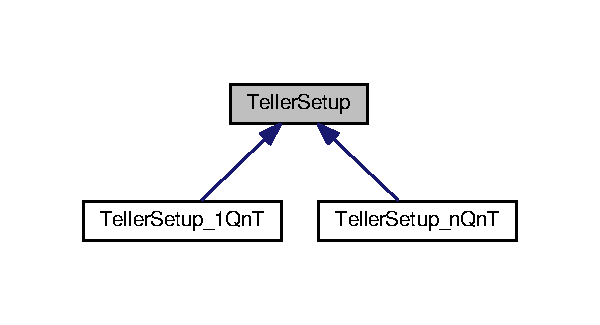
\includegraphics[width=288pt]{class_teller_setup__inherit__graph}
\end{center}
\end{figure}
\subsection*{Public Member Functions}
\begin{DoxyCompactItemize}
\item 
virtual void \hyperlink{class_teller_setup_a2050cd6f277e76cd662b68cf33396034}{simulate} (\hyperlink{class_event_queue}{Event\+Queue} $\ast$p\+Eq)=0
\begin{DoxyCompactList}\small\item\em Run the simulation (1 trial). \end{DoxyCompactList}\item 
void \hyperlink{class_teller_setup_a0a95ca183af3f059b3a78d418f6ce840}{print\+Stats} (std\+::ostream \&out)
\begin{DoxyCompactList}\small\item\em Output setup stats. \end{DoxyCompactList}\end{DoxyCompactItemize}
\subsection*{Protected Attributes}
\begin{DoxyCompactItemize}
\item 
double \hyperlink{class_teller_setup_a173e4329c08235e8c4e9ba2621ccc1fa}{num\+Trials}
\item 
double \hyperlink{class_teller_setup_ae8ef4ccdd294ced6548359d881f86b0a}{tot\+C\+P\+U\+Time}
\item 
double \hyperlink{class_teller_setup_adaeb7d70c8f45a5439f302ff8aaa8f88}{tot\+Virt\+Time}
\item 
double \hyperlink{class_teller_setup_a3eefb44531accf95b6a53351a6fa0998}{tot\+Avg\+Wait\+Time}
\item 
double \hyperlink{class_teller_setup_ac9453ba402c036596a08cb17f32cd117}{tot\+Max\+Wait\+Time}
\item 
double \hyperlink{class_teller_setup_ae8f40bfa4264225d89073489523f5af5}{tot\+Avg\+Line\+Len}
\item 
double \hyperlink{class_teller_setup_af54ac3ef30003e2b568e5b525775c7f2}{tot\+Max\+Line\+Len}
\item 
std\+::vector$<$ double $>$ \hyperlink{class_teller_setup_a9cec8b17536649bf75d13a37ea5d6503}{tot\+Idle\+Time\+Per\+Teller}
\item 
int \hyperlink{class_teller_setup_a13bbfedd5addeb9ee28f08be33d899ae}{num\+Tellers}
\item 
int \hyperlink{class_teller_setup_a4020566b4410400d984ced7c44424390}{num\+Lines}
\end{DoxyCompactItemize}


\subsection{Member Function Documentation}
\index{Teller\+Setup@{Teller\+Setup}!print\+Stats@{print\+Stats}}
\index{print\+Stats@{print\+Stats}!Teller\+Setup@{Teller\+Setup}}
\subsubsection[{\texorpdfstring{print\+Stats(std\+::ostream \&out)}{printStats(std::ostream &out)}}]{\setlength{\rightskip}{0pt plus 5cm}void Teller\+Setup\+::print\+Stats (
\begin{DoxyParamCaption}
\item[{std\+::ostream \&}]{out}
\end{DoxyParamCaption}
)}\hypertarget{class_teller_setup_a0a95ca183af3f059b3a78d418f6ce840}{}\label{class_teller_setup_a0a95ca183af3f059b3a78d418f6ce840}


Output setup stats. 


\begin{DoxyParams}{Parameters}
{\em out} & The stream to write to. \\
\hline
\end{DoxyParams}
\index{Teller\+Setup@{Teller\+Setup}!simulate@{simulate}}
\index{simulate@{simulate}!Teller\+Setup@{Teller\+Setup}}
\subsubsection[{\texorpdfstring{simulate(\+Event\+Queue $\ast$p\+Eq)=0}{simulate(EventQueue *pEq)=0}}]{\setlength{\rightskip}{0pt plus 5cm}virtual void Teller\+Setup\+::simulate (
\begin{DoxyParamCaption}
\item[{{\bf Event\+Queue} $\ast$}]{p\+Eq}
\end{DoxyParamCaption}
)\hspace{0.3cm}{\ttfamily [pure virtual]}}\hypertarget{class_teller_setup_a2050cd6f277e76cd662b68cf33396034}{}\label{class_teller_setup_a2050cd6f277e76cd662b68cf33396034}


Run the simulation (1 trial). 


\begin{DoxyParams}{Parameters}
{\em p\+Eq} & Pointer to the \hyperlink{class_event_queue}{Event\+Queue} of events to feed the simulation. \\
\hline
\end{DoxyParams}


Implemented in \hyperlink{class_teller_setup__1_qn_t_a99b00d1025e46b359f6d1f05f51ebde1}{Teller\+Setup\+\_\+1\+QnT}, and \hyperlink{class_teller_setup__n_qn_t_a2fcbc047bcbdc25f1d123fe65ee80625}{Teller\+Setup\+\_\+n\+QnT}.



\subsection{Member Data Documentation}
\index{Teller\+Setup@{Teller\+Setup}!num\+Lines@{num\+Lines}}
\index{num\+Lines@{num\+Lines}!Teller\+Setup@{Teller\+Setup}}
\subsubsection[{\texorpdfstring{num\+Lines}{numLines}}]{\setlength{\rightskip}{0pt plus 5cm}int Teller\+Setup\+::num\+Lines\hspace{0.3cm}{\ttfamily [protected]}}\hypertarget{class_teller_setup_a4020566b4410400d984ced7c44424390}{}\label{class_teller_setup_a4020566b4410400d984ced7c44424390}
\index{Teller\+Setup@{Teller\+Setup}!num\+Tellers@{num\+Tellers}}
\index{num\+Tellers@{num\+Tellers}!Teller\+Setup@{Teller\+Setup}}
\subsubsection[{\texorpdfstring{num\+Tellers}{numTellers}}]{\setlength{\rightskip}{0pt plus 5cm}int Teller\+Setup\+::num\+Tellers\hspace{0.3cm}{\ttfamily [protected]}}\hypertarget{class_teller_setup_a13bbfedd5addeb9ee28f08be33d899ae}{}\label{class_teller_setup_a13bbfedd5addeb9ee28f08be33d899ae}
\index{Teller\+Setup@{Teller\+Setup}!num\+Trials@{num\+Trials}}
\index{num\+Trials@{num\+Trials}!Teller\+Setup@{Teller\+Setup}}
\subsubsection[{\texorpdfstring{num\+Trials}{numTrials}}]{\setlength{\rightskip}{0pt plus 5cm}double Teller\+Setup\+::num\+Trials\hspace{0.3cm}{\ttfamily [protected]}}\hypertarget{class_teller_setup_a173e4329c08235e8c4e9ba2621ccc1fa}{}\label{class_teller_setup_a173e4329c08235e8c4e9ba2621ccc1fa}
\index{Teller\+Setup@{Teller\+Setup}!tot\+Avg\+Line\+Len@{tot\+Avg\+Line\+Len}}
\index{tot\+Avg\+Line\+Len@{tot\+Avg\+Line\+Len}!Teller\+Setup@{Teller\+Setup}}
\subsubsection[{\texorpdfstring{tot\+Avg\+Line\+Len}{totAvgLineLen}}]{\setlength{\rightskip}{0pt plus 5cm}double Teller\+Setup\+::tot\+Avg\+Line\+Len\hspace{0.3cm}{\ttfamily [protected]}}\hypertarget{class_teller_setup_ae8f40bfa4264225d89073489523f5af5}{}\label{class_teller_setup_ae8f40bfa4264225d89073489523f5af5}
\index{Teller\+Setup@{Teller\+Setup}!tot\+Avg\+Wait\+Time@{tot\+Avg\+Wait\+Time}}
\index{tot\+Avg\+Wait\+Time@{tot\+Avg\+Wait\+Time}!Teller\+Setup@{Teller\+Setup}}
\subsubsection[{\texorpdfstring{tot\+Avg\+Wait\+Time}{totAvgWaitTime}}]{\setlength{\rightskip}{0pt plus 5cm}double Teller\+Setup\+::tot\+Avg\+Wait\+Time\hspace{0.3cm}{\ttfamily [protected]}}\hypertarget{class_teller_setup_a3eefb44531accf95b6a53351a6fa0998}{}\label{class_teller_setup_a3eefb44531accf95b6a53351a6fa0998}
\index{Teller\+Setup@{Teller\+Setup}!tot\+C\+P\+U\+Time@{tot\+C\+P\+U\+Time}}
\index{tot\+C\+P\+U\+Time@{tot\+C\+P\+U\+Time}!Teller\+Setup@{Teller\+Setup}}
\subsubsection[{\texorpdfstring{tot\+C\+P\+U\+Time}{totCPUTime}}]{\setlength{\rightskip}{0pt plus 5cm}double Teller\+Setup\+::tot\+C\+P\+U\+Time\hspace{0.3cm}{\ttfamily [protected]}}\hypertarget{class_teller_setup_ae8ef4ccdd294ced6548359d881f86b0a}{}\label{class_teller_setup_ae8ef4ccdd294ced6548359d881f86b0a}
\index{Teller\+Setup@{Teller\+Setup}!tot\+Idle\+Time\+Per\+Teller@{tot\+Idle\+Time\+Per\+Teller}}
\index{tot\+Idle\+Time\+Per\+Teller@{tot\+Idle\+Time\+Per\+Teller}!Teller\+Setup@{Teller\+Setup}}
\subsubsection[{\texorpdfstring{tot\+Idle\+Time\+Per\+Teller}{totIdleTimePerTeller}}]{\setlength{\rightskip}{0pt plus 5cm}std\+::vector$<$double$>$ Teller\+Setup\+::tot\+Idle\+Time\+Per\+Teller\hspace{0.3cm}{\ttfamily [protected]}}\hypertarget{class_teller_setup_a9cec8b17536649bf75d13a37ea5d6503}{}\label{class_teller_setup_a9cec8b17536649bf75d13a37ea5d6503}
\index{Teller\+Setup@{Teller\+Setup}!tot\+Max\+Line\+Len@{tot\+Max\+Line\+Len}}
\index{tot\+Max\+Line\+Len@{tot\+Max\+Line\+Len}!Teller\+Setup@{Teller\+Setup}}
\subsubsection[{\texorpdfstring{tot\+Max\+Line\+Len}{totMaxLineLen}}]{\setlength{\rightskip}{0pt plus 5cm}double Teller\+Setup\+::tot\+Max\+Line\+Len\hspace{0.3cm}{\ttfamily [protected]}}\hypertarget{class_teller_setup_af54ac3ef30003e2b568e5b525775c7f2}{}\label{class_teller_setup_af54ac3ef30003e2b568e5b525775c7f2}
\index{Teller\+Setup@{Teller\+Setup}!tot\+Max\+Wait\+Time@{tot\+Max\+Wait\+Time}}
\index{tot\+Max\+Wait\+Time@{tot\+Max\+Wait\+Time}!Teller\+Setup@{Teller\+Setup}}
\subsubsection[{\texorpdfstring{tot\+Max\+Wait\+Time}{totMaxWaitTime}}]{\setlength{\rightskip}{0pt plus 5cm}double Teller\+Setup\+::tot\+Max\+Wait\+Time\hspace{0.3cm}{\ttfamily [protected]}}\hypertarget{class_teller_setup_ac9453ba402c036596a08cb17f32cd117}{}\label{class_teller_setup_ac9453ba402c036596a08cb17f32cd117}
\index{Teller\+Setup@{Teller\+Setup}!tot\+Virt\+Time@{tot\+Virt\+Time}}
\index{tot\+Virt\+Time@{tot\+Virt\+Time}!Teller\+Setup@{Teller\+Setup}}
\subsubsection[{\texorpdfstring{tot\+Virt\+Time}{totVirtTime}}]{\setlength{\rightskip}{0pt plus 5cm}double Teller\+Setup\+::tot\+Virt\+Time\hspace{0.3cm}{\ttfamily [protected]}}\hypertarget{class_teller_setup_adaeb7d70c8f45a5439f302ff8aaa8f88}{}\label{class_teller_setup_adaeb7d70c8f45a5439f302ff8aaa8f88}


The documentation for this class was generated from the following files\+:\begin{DoxyCompactItemize}
\item 
\hyperlink{_teller_setup_8h}{Teller\+Setup.\+h}\item 
\hyperlink{_teller_setup_8cpp}{Teller\+Setup.\+cpp}\end{DoxyCompactItemize}

\hypertarget{class_teller_setup__1_qn_t}{}\section{Teller\+Setup\+\_\+1\+QnT Class Reference}
\label{class_teller_setup__1_qn_t}\index{Teller\+Setup\+\_\+1\+QnT@{Teller\+Setup\+\_\+1\+QnT}}


{\ttfamily \#include $<$Teller\+Setup\+\_\+1\+Qn\+T.\+h$>$}



Inheritance diagram for Teller\+Setup\+\_\+1\+QnT\+:
\nopagebreak
\begin{figure}[H]
\begin{center}
\leavevmode
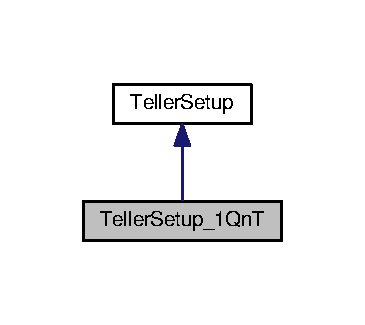
\includegraphics[width=175pt]{class_teller_setup__1_qn_t__inherit__graph}
\end{center}
\end{figure}


Collaboration diagram for Teller\+Setup\+\_\+1\+QnT\+:
\nopagebreak
\begin{figure}[H]
\begin{center}
\leavevmode
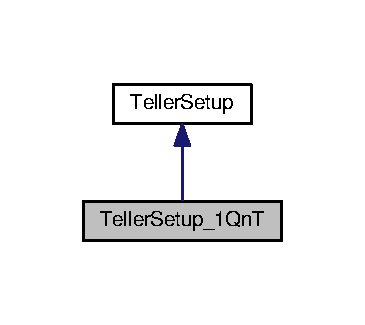
\includegraphics[width=175pt]{class_teller_setup__1_qn_t__coll__graph}
\end{center}
\end{figure}
\subsection*{Public Member Functions}
\begin{DoxyCompactItemize}
\item 
\hyperlink{class_teller_setup__1_qn_t_a811d35eefb095b4907605596a99a444b}{Teller\+Setup\+\_\+1\+QnT} (int n)
\begin{DoxyCompactList}\small\item\em Constructs a 1\+QnT \hyperlink{class_teller}{Teller} Setup with given n. \end{DoxyCompactList}\item 
void \hyperlink{class_teller_setup__1_qn_t_a99b00d1025e46b359f6d1f05f51ebde1}{simulate} (\hyperlink{class_event_queue}{Event\+Queue} $\ast$p\+Eq)
\end{DoxyCompactItemize}
\subsection*{Additional Inherited Members}


\subsection{Constructor \& Destructor Documentation}
\index{Teller\+Setup\+\_\+1\+QnT@{Teller\+Setup\+\_\+1\+QnT}!Teller\+Setup\+\_\+1\+QnT@{Teller\+Setup\+\_\+1\+QnT}}
\index{Teller\+Setup\+\_\+1\+QnT@{Teller\+Setup\+\_\+1\+QnT}!Teller\+Setup\+\_\+1\+QnT@{Teller\+Setup\+\_\+1\+QnT}}
\subsubsection[{\texorpdfstring{Teller\+Setup\+\_\+1\+Qn\+T(int n)}{TellerSetup_1QnT(int n)}}]{\setlength{\rightskip}{0pt plus 5cm}Teller\+Setup\+\_\+1\+Qn\+T\+::\+Teller\+Setup\+\_\+1\+QnT (
\begin{DoxyParamCaption}
\item[{int}]{n}
\end{DoxyParamCaption}
)}\hypertarget{class_teller_setup__1_qn_t_a811d35eefb095b4907605596a99a444b}{}\label{class_teller_setup__1_qn_t_a811d35eefb095b4907605596a99a444b}


Constructs a 1\+QnT \hyperlink{class_teller}{Teller} Setup with given n. 


\begin{DoxyParams}{Parameters}
{\em n} & The number of tellers. \\
\hline
\end{DoxyParams}


\subsection{Member Function Documentation}
\index{Teller\+Setup\+\_\+1\+QnT@{Teller\+Setup\+\_\+1\+QnT}!simulate@{simulate}}
\index{simulate@{simulate}!Teller\+Setup\+\_\+1\+QnT@{Teller\+Setup\+\_\+1\+QnT}}
\subsubsection[{\texorpdfstring{simulate(\+Event\+Queue $\ast$p\+Eq)}{simulate(EventQueue *pEq)}}]{\setlength{\rightskip}{0pt plus 5cm}void Teller\+Setup\+\_\+1\+Qn\+T\+::simulate (
\begin{DoxyParamCaption}
\item[{{\bf Event\+Queue} $\ast$}]{p\+Eq}
\end{DoxyParamCaption}
)\hspace{0.3cm}{\ttfamily [virtual]}}\hypertarget{class_teller_setup__1_qn_t_a99b00d1025e46b359f6d1f05f51ebde1}{}\label{class_teller_setup__1_qn_t_a99b00d1025e46b359f6d1f05f51ebde1}
Run the simulation (1 trial). 

Implements \hyperlink{class_teller_setup_a2050cd6f277e76cd662b68cf33396034}{Teller\+Setup}.



The documentation for this class was generated from the following files\+:\begin{DoxyCompactItemize}
\item 
\hyperlink{_teller_setup__1_qn_t_8h}{Teller\+Setup\+\_\+1\+Qn\+T.\+h}\item 
\hyperlink{_teller_setup__1_qn_t_8cpp}{Teller\+Setup\+\_\+1\+Qn\+T.\+cpp}\end{DoxyCompactItemize}

\hypertarget{class_teller_setup__n_qn_t}{}\section{Teller\+Setup\+\_\+n\+QnT Class Reference}
\label{class_teller_setup__n_qn_t}\index{Teller\+Setup\+\_\+n\+QnT@{Teller\+Setup\+\_\+n\+QnT}}


{\ttfamily \#include $<$Teller\+Setup\+\_\+n\+Qn\+T.\+h$>$}



Inheritance diagram for Teller\+Setup\+\_\+n\+QnT\+:
\nopagebreak
\begin{figure}[H]
\begin{center}
\leavevmode
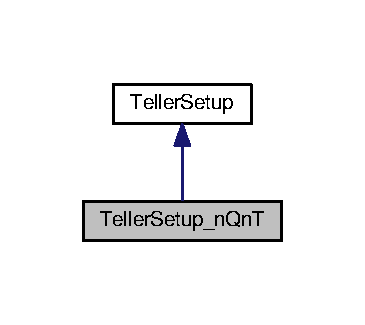
\includegraphics[width=175pt]{class_teller_setup__n_qn_t__inherit__graph}
\end{center}
\end{figure}


Collaboration diagram for Teller\+Setup\+\_\+n\+QnT\+:
\nopagebreak
\begin{figure}[H]
\begin{center}
\leavevmode
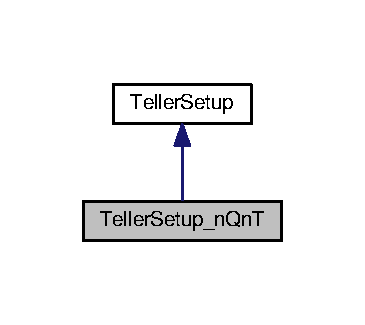
\includegraphics[width=175pt]{class_teller_setup__n_qn_t__coll__graph}
\end{center}
\end{figure}
\subsection*{Public Member Functions}
\begin{DoxyCompactItemize}
\item 
\hyperlink{class_teller_setup__n_qn_t_aa76a1c946ba54abc4930f6aeee69f229}{Teller\+Setup\+\_\+n\+QnT} (int n)
\begin{DoxyCompactList}\small\item\em Constructs a n\+QnT \hyperlink{class_teller}{Teller} Setup with given n. \end{DoxyCompactList}\item 
void \hyperlink{class_teller_setup__n_qn_t_a2fcbc047bcbdc25f1d123fe65ee80625}{simulate} (\hyperlink{class_event_queue}{Event\+Queue} $\ast$p\+Eq)
\end{DoxyCompactItemize}
\subsection*{Additional Inherited Members}


\subsection{Constructor \& Destructor Documentation}
\index{Teller\+Setup\+\_\+n\+QnT@{Teller\+Setup\+\_\+n\+QnT}!Teller\+Setup\+\_\+n\+QnT@{Teller\+Setup\+\_\+n\+QnT}}
\index{Teller\+Setup\+\_\+n\+QnT@{Teller\+Setup\+\_\+n\+QnT}!Teller\+Setup\+\_\+n\+QnT@{Teller\+Setup\+\_\+n\+QnT}}
\subsubsection[{\texorpdfstring{Teller\+Setup\+\_\+n\+Qn\+T(int n)}{TellerSetup_nQnT(int n)}}]{\setlength{\rightskip}{0pt plus 5cm}Teller\+Setup\+\_\+n\+Qn\+T\+::\+Teller\+Setup\+\_\+n\+QnT (
\begin{DoxyParamCaption}
\item[{int}]{n}
\end{DoxyParamCaption}
)}\hypertarget{class_teller_setup__n_qn_t_aa76a1c946ba54abc4930f6aeee69f229}{}\label{class_teller_setup__n_qn_t_aa76a1c946ba54abc4930f6aeee69f229}


Constructs a n\+QnT \hyperlink{class_teller}{Teller} Setup with given n. 


\begin{DoxyParams}{Parameters}
{\em n} & The number of tellers and queues. \\
\hline
\end{DoxyParams}


\subsection{Member Function Documentation}
\index{Teller\+Setup\+\_\+n\+QnT@{Teller\+Setup\+\_\+n\+QnT}!simulate@{simulate}}
\index{simulate@{simulate}!Teller\+Setup\+\_\+n\+QnT@{Teller\+Setup\+\_\+n\+QnT}}
\subsubsection[{\texorpdfstring{simulate(\+Event\+Queue $\ast$p\+Eq)}{simulate(EventQueue *pEq)}}]{\setlength{\rightskip}{0pt plus 5cm}void Teller\+Setup\+\_\+n\+Qn\+T\+::simulate (
\begin{DoxyParamCaption}
\item[{{\bf Event\+Queue} $\ast$}]{p\+Eq}
\end{DoxyParamCaption}
)\hspace{0.3cm}{\ttfamily [virtual]}}\hypertarget{class_teller_setup__n_qn_t_a2fcbc047bcbdc25f1d123fe65ee80625}{}\label{class_teller_setup__n_qn_t_a2fcbc047bcbdc25f1d123fe65ee80625}
Run the simulation (1 trial). 

Implements \hyperlink{class_teller_setup_a2050cd6f277e76cd662b68cf33396034}{Teller\+Setup}.



The documentation for this class was generated from the following files\+:\begin{DoxyCompactItemize}
\item 
\hyperlink{_teller_setup__n_qn_t_8h}{Teller\+Setup\+\_\+n\+Qn\+T.\+h}\item 
\hyperlink{_teller_setup__n_qn_t_8cpp}{Teller\+Setup\+\_\+n\+Qn\+T.\+cpp}\end{DoxyCompactItemize}

\hypertarget{class_tickable}{}\section{Tickable Class Reference}
\label{class_tickable}\index{Tickable@{Tickable}}


A \hyperlink{class_tickable}{Tickable} object.  




{\ttfamily \#include $<$Teller\+Setup.\+h$>$}



Inheritance diagram for Tickable\+:
\nopagebreak
\begin{figure}[H]
\begin{center}
\leavevmode
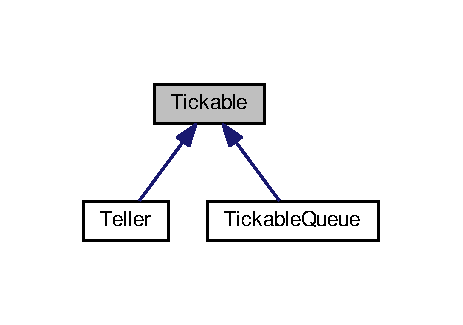
\includegraphics[width=222pt]{class_tickable__inherit__graph}
\end{center}
\end{figure}
\subsection*{Public Member Functions}
\begin{DoxyCompactItemize}
\item 
virtual void \hyperlink{class_tickable_a0ca181a29c3e1539e4221d2cbcfa83c2}{tick} (int now)=0
\begin{DoxyCompactList}\small\item\em Do one tick at the given time. \end{DoxyCompactList}\item 
virtual int \hyperlink{class_tickable_ac65be54f32d39d1450a37cf4acb1ad15}{when\+Next} ()=0
\begin{DoxyCompactList}\small\item\em Get when this tickable needs to be ticked next. \end{DoxyCompactList}\end{DoxyCompactItemize}


\subsection{Detailed Description}
A \hyperlink{class_tickable}{Tickable} object. 

For use by \hyperlink{class_teller_setup}{Teller\+Setup}. 

\subsection{Member Function Documentation}
\index{Tickable@{Tickable}!tick@{tick}}
\index{tick@{tick}!Tickable@{Tickable}}
\subsubsection[{\texorpdfstring{tick(int now)=0}{tick(int now)=0}}]{\setlength{\rightskip}{0pt plus 5cm}virtual void Tickable\+::tick (
\begin{DoxyParamCaption}
\item[{int}]{now}
\end{DoxyParamCaption}
)\hspace{0.3cm}{\ttfamily [pure virtual]}}\hypertarget{class_tickable_a0ca181a29c3e1539e4221d2cbcfa83c2}{}\label{class_tickable_a0ca181a29c3e1539e4221d2cbcfa83c2}


Do one tick at the given time. 


\begin{DoxyParams}{Parameters}
{\em now} & The current time. \\
\hline
\end{DoxyParams}


Implemented in \hyperlink{class_tickable_queue_afabd7085cb5f7cba4286246d69f42211}{Tickable\+Queue}, and \hyperlink{class_teller_aa8cf7bb201a88b959b42a3c4358565c3}{Teller}.

\index{Tickable@{Tickable}!when\+Next@{when\+Next}}
\index{when\+Next@{when\+Next}!Tickable@{Tickable}}
\subsubsection[{\texorpdfstring{when\+Next()=0}{whenNext()=0}}]{\setlength{\rightskip}{0pt plus 5cm}virtual int Tickable\+::when\+Next (
\begin{DoxyParamCaption}
{}
\end{DoxyParamCaption}
)\hspace{0.3cm}{\ttfamily [pure virtual]}}\hypertarget{class_tickable_ac65be54f32d39d1450a37cf4acb1ad15}{}\label{class_tickable_ac65be54f32d39d1450a37cf4acb1ad15}


Get when this tickable needs to be ticked next. 

Returns -\/1 when there is no future event. \begin{DoxyReturn}{Returns}
When this tickable needs to be ticked next. 
\end{DoxyReturn}


Implemented in \hyperlink{class_tickable_queue_a7ce766623b9b1610147b920018de5066}{Tickable\+Queue}, and \hyperlink{class_teller_a10106b3a286c21870bde1751aec0f9b6}{Teller}.



The documentation for this class was generated from the following file\+:\begin{DoxyCompactItemize}
\item 
\hyperlink{_teller_setup_8h}{Teller\+Setup.\+h}\end{DoxyCompactItemize}

\hypertarget{class_tickable_queue}{}\section{Tickable\+Queue Class Reference}
\label{class_tickable_queue}\index{Tickable\+Queue@{Tickable\+Queue}}


An \hyperlink{class_event_queue}{Event\+Queue} wrapper that enables tick functionality.  




{\ttfamily \#include $<$Teller\+Setup.\+h$>$}



Inheritance diagram for Tickable\+Queue\+:
\nopagebreak
\begin{figure}[H]
\begin{center}
\leavevmode
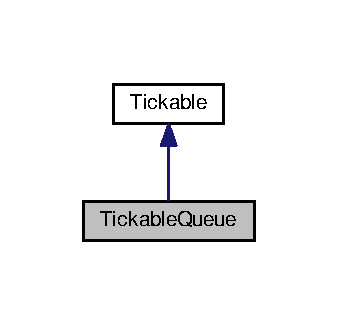
\includegraphics[width=162pt]{class_tickable_queue__inherit__graph}
\end{center}
\end{figure}


Collaboration diagram for Tickable\+Queue\+:
\nopagebreak
\begin{figure}[H]
\begin{center}
\leavevmode
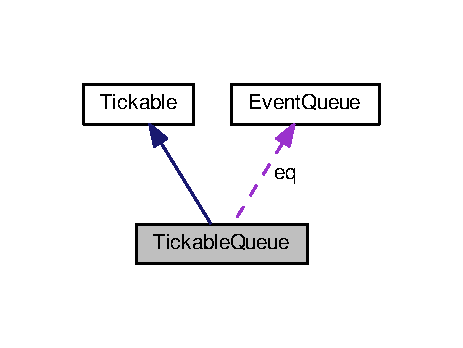
\includegraphics[width=222pt]{class_tickable_queue__coll__graph}
\end{center}
\end{figure}
\subsection*{Public Member Functions}
\begin{DoxyCompactItemize}
\item 
\hyperlink{class_tickable_queue_ae4bc32b25ba1dc036173444df9c92d91}{Tickable\+Queue} (\hyperlink{class_event_queue}{Event\+Queue} $\ast$evQ, double $\ast$tll, double $\ast$mll)
\begin{DoxyCompactList}\small\item\em Constructs a \hyperlink{class_tickable_queue}{Tickable\+Queue} around the given \hyperlink{class_event_queue}{Event\+Queue}. \end{DoxyCompactList}\item 
void \hyperlink{class_tickable_queue_ac0a0fb1ed5312a1e93f471ae12e0238e}{reg\+Dest\+Queue} (\hyperlink{class_event_queue}{Event\+Queue} $\ast$dest)
\begin{DoxyCompactList}\small\item\em Register a destination queue for this queue to feed into. \end{DoxyCompactList}\item 
void \hyperlink{class_tickable_queue_afabd7085cb5f7cba4286246d69f42211}{tick} (int now)
\item 
int \hyperlink{class_tickable_queue_a7ce766623b9b1610147b920018de5066}{when\+Next} ()
\end{DoxyCompactItemize}
\subsection*{Private Attributes}
\begin{DoxyCompactItemize}
\item 
\hyperlink{class_event_queue}{Event\+Queue} $\ast$ \hyperlink{class_tickable_queue_ad14bee370bdfb8db2550fa3fd7a11a3a}{eq}
\item 
std\+::vector$<$ \hyperlink{class_event_queue}{Event\+Queue} $\ast$ $>$ \hyperlink{class_tickable_queue_a44b1ef6bc662fc500030f35a4f10e73a}{dest\+Lines}
\item 
double $\ast$ \hyperlink{class_tickable_queue_a29b6a86071a7c56798a5a8633435260e}{tot\+Line\+Len}
\item 
double $\ast$ \hyperlink{class_tickable_queue_a86b7e60ef45f0405279725058820f4a8}{max\+Line\+Len}
\item 
int \hyperlink{class_tickable_queue_a1bab2d5f40fb2a9f8ba171239843f422}{last\+Ticked}
\end{DoxyCompactItemize}


\subsection{Detailed Description}
An \hyperlink{class_event_queue}{Event\+Queue} wrapper that enables tick functionality. 

An \hyperlink{class_event_queue}{Event\+Queue} wrapper that can be \char`\"{}ticked\char`\"{}. 

\subsection{Constructor \& Destructor Documentation}
\index{Tickable\+Queue@{Tickable\+Queue}!Tickable\+Queue@{Tickable\+Queue}}
\index{Tickable\+Queue@{Tickable\+Queue}!Tickable\+Queue@{Tickable\+Queue}}
\subsubsection[{\texorpdfstring{Tickable\+Queue(\+Event\+Queue $\ast$ev\+Q, double $\ast$tll, double $\ast$mll)}{TickableQueue(EventQueue *evQ, double *tll, double *mll)}}]{\setlength{\rightskip}{0pt plus 5cm}Tickable\+Queue\+::\+Tickable\+Queue (
\begin{DoxyParamCaption}
\item[{{\bf Event\+Queue} $\ast$}]{evQ, }
\item[{double $\ast$}]{tll, }
\item[{double $\ast$}]{mll}
\end{DoxyParamCaption}
)}\hypertarget{class_tickable_queue_ae4bc32b25ba1dc036173444df9c92d91}{}\label{class_tickable_queue_ae4bc32b25ba1dc036173444df9c92d91}


Constructs a \hyperlink{class_tickable_queue}{Tickable\+Queue} around the given \hyperlink{class_event_queue}{Event\+Queue}. 


\begin{DoxyParams}{Parameters}
{\em evQ} & The \hyperlink{class_event_queue}{Event\+Queue} to wrap. \\
\hline
{\em tll} & Pointer to the total line length over time counter. \\
\hline
{\em mll} & Pointer to the max line length counter. \\
\hline
\end{DoxyParams}


\subsection{Member Function Documentation}
\index{Tickable\+Queue@{Tickable\+Queue}!reg\+Dest\+Queue@{reg\+Dest\+Queue}}
\index{reg\+Dest\+Queue@{reg\+Dest\+Queue}!Tickable\+Queue@{Tickable\+Queue}}
\subsubsection[{\texorpdfstring{reg\+Dest\+Queue(\+Event\+Queue $\ast$dest)}{regDestQueue(EventQueue *dest)}}]{\setlength{\rightskip}{0pt plus 5cm}void Tickable\+Queue\+::reg\+Dest\+Queue (
\begin{DoxyParamCaption}
\item[{{\bf Event\+Queue} $\ast$}]{dest}
\end{DoxyParamCaption}
)}\hypertarget{class_tickable_queue_ac0a0fb1ed5312a1e93f471ae12e0238e}{}\label{class_tickable_queue_ac0a0fb1ed5312a1e93f471ae12e0238e}


Register a destination queue for this queue to feed into. 


\begin{DoxyParams}{Parameters}
{\em dest} & The queue to register. \\
\hline
\end{DoxyParams}
\index{Tickable\+Queue@{Tickable\+Queue}!tick@{tick}}
\index{tick@{tick}!Tickable\+Queue@{Tickable\+Queue}}
\subsubsection[{\texorpdfstring{tick(int now)}{tick(int now)}}]{\setlength{\rightskip}{0pt plus 5cm}void Tickable\+Queue\+::tick (
\begin{DoxyParamCaption}
\item[{int}]{now}
\end{DoxyParamCaption}
)\hspace{0.3cm}{\ttfamily [virtual]}}\hypertarget{class_tickable_queue_afabd7085cb5f7cba4286246d69f42211}{}\label{class_tickable_queue_afabd7085cb5f7cba4286246d69f42211}
Do one tick at the given time. 

Implements \hyperlink{class_tickable_a0ca181a29c3e1539e4221d2cbcfa83c2}{Tickable}.

\index{Tickable\+Queue@{Tickable\+Queue}!when\+Next@{when\+Next}}
\index{when\+Next@{when\+Next}!Tickable\+Queue@{Tickable\+Queue}}
\subsubsection[{\texorpdfstring{when\+Next()}{whenNext()}}]{\setlength{\rightskip}{0pt plus 5cm}int Tickable\+Queue\+::when\+Next (
\begin{DoxyParamCaption}
{}
\end{DoxyParamCaption}
)\hspace{0.3cm}{\ttfamily [virtual]}}\hypertarget{class_tickable_queue_a7ce766623b9b1610147b920018de5066}{}\label{class_tickable_queue_a7ce766623b9b1610147b920018de5066}
Get when this tickable needs to be ticked next. 

Implements \hyperlink{class_tickable_ac65be54f32d39d1450a37cf4acb1ad15}{Tickable}.



\subsection{Member Data Documentation}
\index{Tickable\+Queue@{Tickable\+Queue}!dest\+Lines@{dest\+Lines}}
\index{dest\+Lines@{dest\+Lines}!Tickable\+Queue@{Tickable\+Queue}}
\subsubsection[{\texorpdfstring{dest\+Lines}{destLines}}]{\setlength{\rightskip}{0pt plus 5cm}std\+::vector$<${\bf Event\+Queue}$\ast$$>$ Tickable\+Queue\+::dest\+Lines\hspace{0.3cm}{\ttfamily [private]}}\hypertarget{class_tickable_queue_a44b1ef6bc662fc500030f35a4f10e73a}{}\label{class_tickable_queue_a44b1ef6bc662fc500030f35a4f10e73a}
\index{Tickable\+Queue@{Tickable\+Queue}!eq@{eq}}
\index{eq@{eq}!Tickable\+Queue@{Tickable\+Queue}}
\subsubsection[{\texorpdfstring{eq}{eq}}]{\setlength{\rightskip}{0pt plus 5cm}{\bf Event\+Queue}$\ast$ Tickable\+Queue\+::eq\hspace{0.3cm}{\ttfamily [private]}}\hypertarget{class_tickable_queue_ad14bee370bdfb8db2550fa3fd7a11a3a}{}\label{class_tickable_queue_ad14bee370bdfb8db2550fa3fd7a11a3a}
\index{Tickable\+Queue@{Tickable\+Queue}!last\+Ticked@{last\+Ticked}}
\index{last\+Ticked@{last\+Ticked}!Tickable\+Queue@{Tickable\+Queue}}
\subsubsection[{\texorpdfstring{last\+Ticked}{lastTicked}}]{\setlength{\rightskip}{0pt plus 5cm}int Tickable\+Queue\+::last\+Ticked\hspace{0.3cm}{\ttfamily [private]}}\hypertarget{class_tickable_queue_a1bab2d5f40fb2a9f8ba171239843f422}{}\label{class_tickable_queue_a1bab2d5f40fb2a9f8ba171239843f422}
\index{Tickable\+Queue@{Tickable\+Queue}!max\+Line\+Len@{max\+Line\+Len}}
\index{max\+Line\+Len@{max\+Line\+Len}!Tickable\+Queue@{Tickable\+Queue}}
\subsubsection[{\texorpdfstring{max\+Line\+Len}{maxLineLen}}]{\setlength{\rightskip}{0pt plus 5cm}double$\ast$ Tickable\+Queue\+::max\+Line\+Len\hspace{0.3cm}{\ttfamily [private]}}\hypertarget{class_tickable_queue_a86b7e60ef45f0405279725058820f4a8}{}\label{class_tickable_queue_a86b7e60ef45f0405279725058820f4a8}
\index{Tickable\+Queue@{Tickable\+Queue}!tot\+Line\+Len@{tot\+Line\+Len}}
\index{tot\+Line\+Len@{tot\+Line\+Len}!Tickable\+Queue@{Tickable\+Queue}}
\subsubsection[{\texorpdfstring{tot\+Line\+Len}{totLineLen}}]{\setlength{\rightskip}{0pt plus 5cm}double$\ast$ Tickable\+Queue\+::tot\+Line\+Len\hspace{0.3cm}{\ttfamily [private]}}\hypertarget{class_tickable_queue_a29b6a86071a7c56798a5a8633435260e}{}\label{class_tickable_queue_a29b6a86071a7c56798a5a8633435260e}


The documentation for this class was generated from the following files\+:\begin{DoxyCompactItemize}
\item 
\hyperlink{_teller_setup_8h}{Teller\+Setup.\+h}\item 
\hyperlink{_teller_setup_8cpp}{Teller\+Setup.\+cpp}\end{DoxyCompactItemize}

\chapter{File Documentation}
\hypertarget{_a_b_event_queue_8cpp}{}\section{A\+B\+Event\+Queue.\+cpp File Reference}
\label{_a_b_event_queue_8cpp}\index{A\+B\+Event\+Queue.\+cpp@{A\+B\+Event\+Queue.\+cpp}}
{\ttfamily \#include \char`\"{}A\+B\+Event\+Queue.\+h\char`\"{}}\\*
{\ttfamily \#include $<$string.\+h$>$}\\*
{\ttfamily \#include $<$string$>$}\\*
{\ttfamily \#include $<$iostream$>$}\\*
Include dependency graph for A\+B\+Event\+Queue.\+cpp\+:
\nopagebreak
\begin{figure}[H]
\begin{center}
\leavevmode
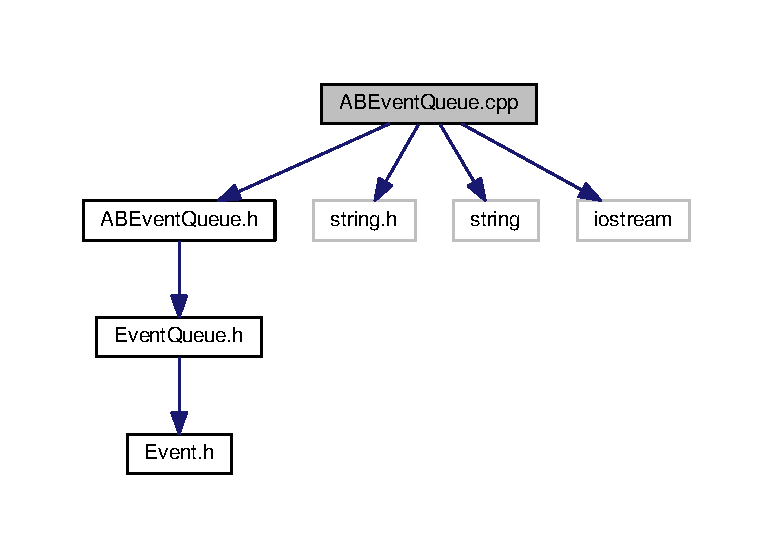
\includegraphics[width=350pt]{_a_b_event_queue_8cpp__incl}
\end{center}
\end{figure}

\hypertarget{_a_b_event_queue_8h}{}\section{A\+B\+Event\+Queue.\+h File Reference}
\label{_a_b_event_queue_8h}\index{A\+B\+Event\+Queue.\+h@{A\+B\+Event\+Queue.\+h}}


Declares the Array-\/\+Based \hyperlink{struct_event}{Event} Queue class.  


{\ttfamily \#include \char`\"{}Event\+Queue.\+h\char`\"{}}\\*
Include dependency graph for A\+B\+Event\+Queue.\+h\+:
\nopagebreak
\begin{figure}[H]
\begin{center}
\leavevmode
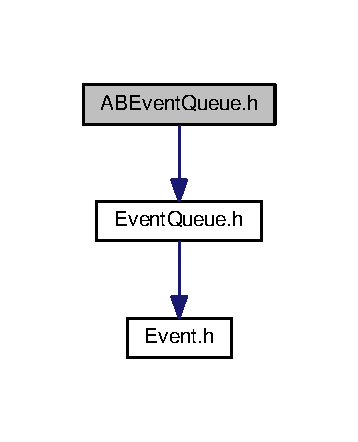
\includegraphics[width=172pt]{_a_b_event_queue_8h__incl}
\end{center}
\end{figure}
This graph shows which files directly or indirectly include this file\+:
\nopagebreak
\begin{figure}[H]
\begin{center}
\leavevmode
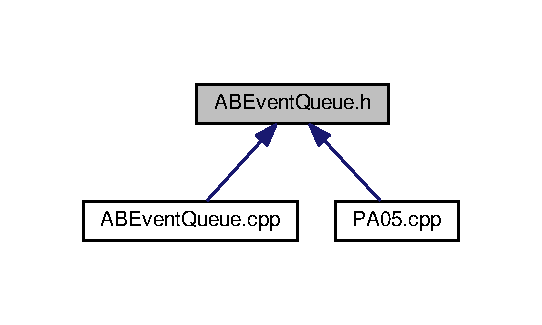
\includegraphics[width=260pt]{_a_b_event_queue_8h__dep__incl}
\end{center}
\end{figure}
\subsection*{Classes}
\begin{DoxyCompactItemize}
\item 
class \hyperlink{class_a_b_event_queue}{A\+B\+Event\+Queue}
\begin{DoxyCompactList}\small\item\em An Array-\/\+Based \hyperlink{struct_event}{Event} Queue. \end{DoxyCompactList}\end{DoxyCompactItemize}


\subsection{Detailed Description}
Declares the Array-\/\+Based \hyperlink{struct_event}{Event} Queue class. 

\begin{DoxyAuthor}{Author}
Matthew Bauer 
\end{DoxyAuthor}

\hypertarget{_event_8h}{}\section{Event.\+h File Reference}
\label{_event_8h}\index{Event.\+h@{Event.\+h}}


Declares the \hyperlink{struct_event}{Event} structure.  


This graph shows which files directly or indirectly include this file\+:
\nopagebreak
\begin{figure}[H]
\begin{center}
\leavevmode
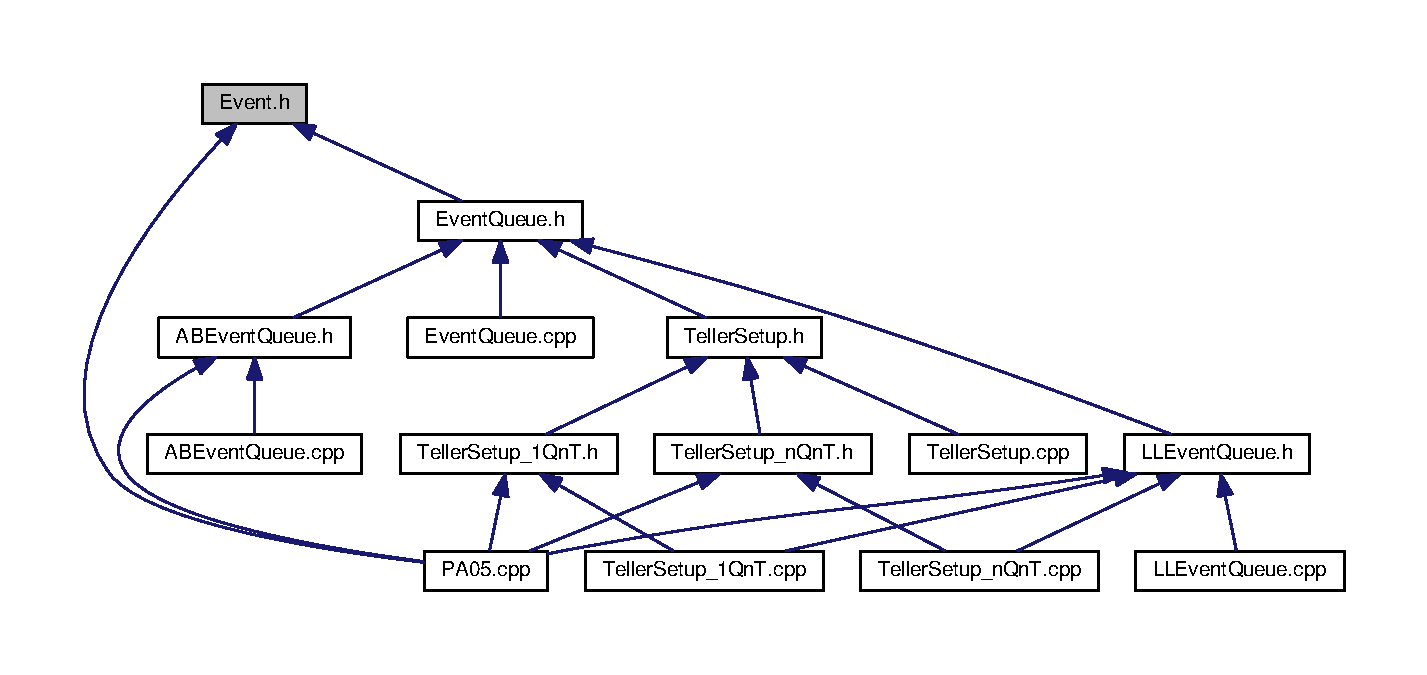
\includegraphics[width=350pt]{_event_8h__dep__incl}
\end{center}
\end{figure}
\subsection*{Classes}
\begin{DoxyCompactItemize}
\item 
struct \hyperlink{struct_event}{Event}
\end{DoxyCompactItemize}


\subsection{Detailed Description}
Declares the \hyperlink{struct_event}{Event} structure. 

\begin{DoxyAuthor}{Author}
Matthew Bauer 
\end{DoxyAuthor}

\hypertarget{_event_queue_8cpp}{}\section{Event\+Queue.\+cpp File Reference}
\label{_event_queue_8cpp}\index{Event\+Queue.\+cpp@{Event\+Queue.\+cpp}}
{\ttfamily \#include \char`\"{}Event\+Queue.\+h\char`\"{}}\\*
{\ttfamily \#include $<$cstdlib$>$}\\*
{\ttfamily \#include $<$algorithm$>$}\\*
{\ttfamily \#include $<$iostream$>$}\\*
Include dependency graph for Event\+Queue.\+cpp\+:
\nopagebreak
\begin{figure}[H]
\begin{center}
\leavevmode
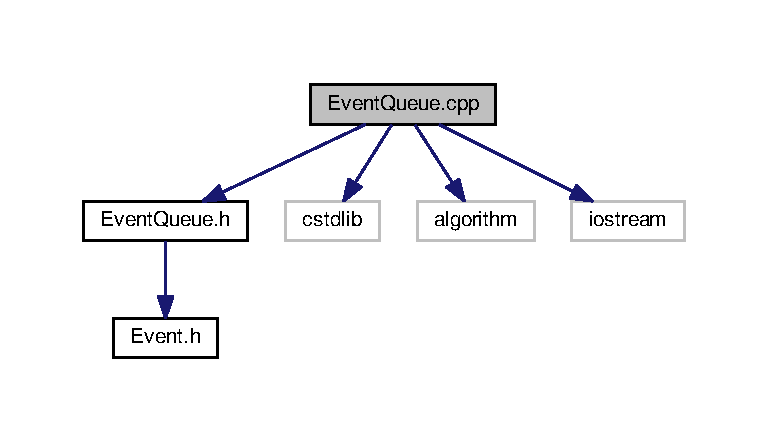
\includegraphics[width=350pt]{_event_queue_8cpp__incl}
\end{center}
\end{figure}

\hypertarget{_event_queue_8h}{}\section{Event\+Queue.\+h File Reference}
\label{_event_queue_8h}\index{Event\+Queue.\+h@{Event\+Queue.\+h}}


Declares the \hyperlink{class_event_queue}{Event\+Queue} abstract class.  


{\ttfamily \#include \char`\"{}Event.\+h\char`\"{}}\\*
Include dependency graph for Event\+Queue.\+h\+:
\nopagebreak
\begin{figure}[H]
\begin{center}
\leavevmode
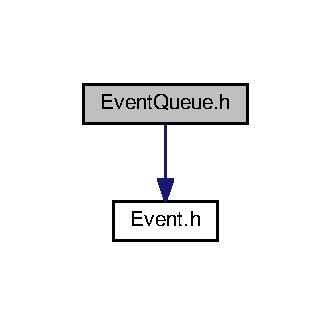
\includegraphics[width=159pt]{_event_queue_8h__incl}
\end{center}
\end{figure}
This graph shows which files directly or indirectly include this file\+:
\nopagebreak
\begin{figure}[H]
\begin{center}
\leavevmode
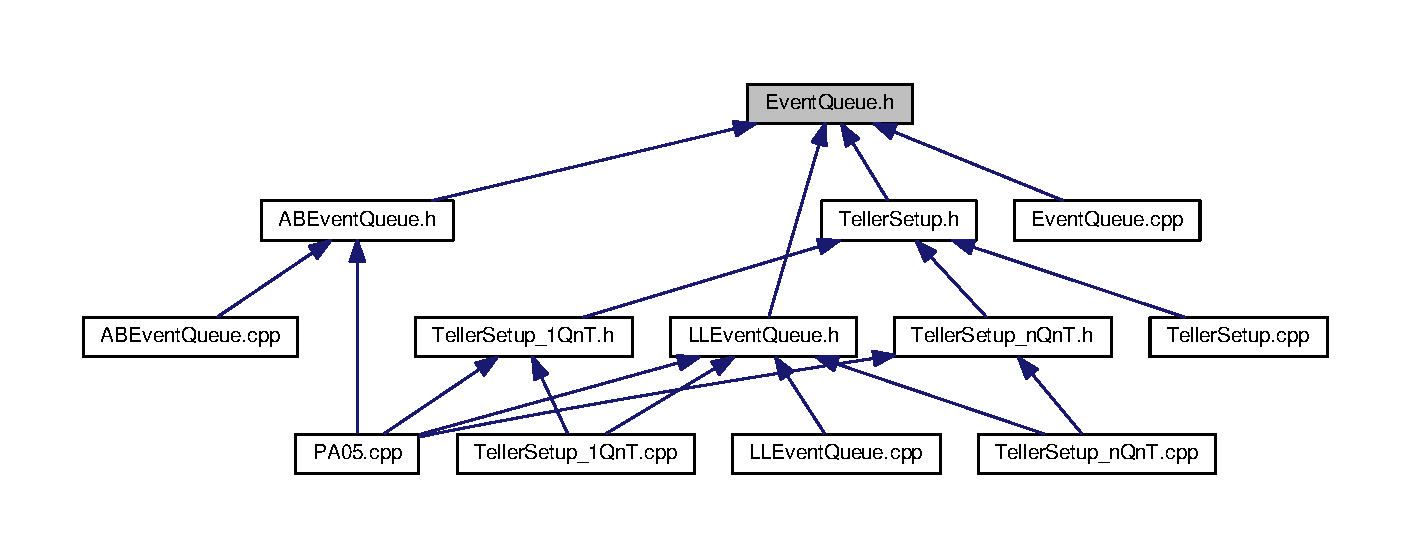
\includegraphics[width=350pt]{_event_queue_8h__dep__incl}
\end{center}
\end{figure}
\subsection*{Classes}
\begin{DoxyCompactItemize}
\item 
class \hyperlink{class_event_queue}{Event\+Queue}
\end{DoxyCompactItemize}


\subsection{Detailed Description}
Declares the \hyperlink{class_event_queue}{Event\+Queue} abstract class. 

\begin{DoxyAuthor}{Author}
Matthew Bauer 
\end{DoxyAuthor}

\hypertarget{_l_l_event_queue_8cpp}{}\section{L\+L\+Event\+Queue.\+cpp File Reference}
\label{_l_l_event_queue_8cpp}\index{L\+L\+Event\+Queue.\+cpp@{L\+L\+Event\+Queue.\+cpp}}
{\ttfamily \#include \char`\"{}L\+L\+Event\+Queue.\+h\char`\"{}}\\*
{\ttfamily \#include $<$string$>$}\\*
Include dependency graph for L\+L\+Event\+Queue.\+cpp\+:
\nopagebreak
\begin{figure}[H]
\begin{center}
\leavevmode
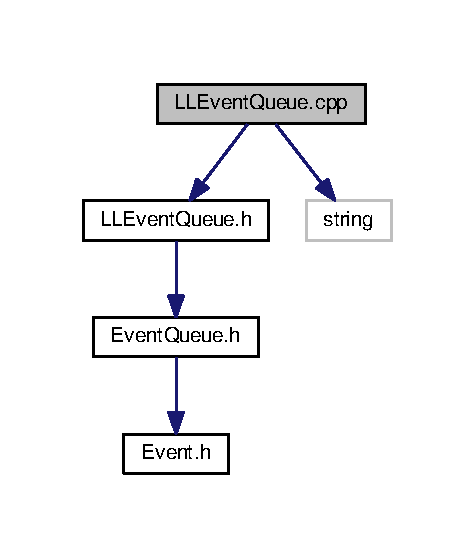
\includegraphics[width=228pt]{_l_l_event_queue_8cpp__incl}
\end{center}
\end{figure}

\hypertarget{_l_l_event_queue_8h}{}\section{L\+L\+Event\+Queue.\+h File Reference}
\label{_l_l_event_queue_8h}\index{L\+L\+Event\+Queue.\+h@{L\+L\+Event\+Queue.\+h}}


Declares the Linked-\/\+List-\/\+Based \hyperlink{struct_event}{Event} Queue class.  


{\ttfamily \#include \char`\"{}Event\+Queue.\+h\char`\"{}}\\*
Include dependency graph for L\+L\+Event\+Queue.\+h\+:
\nopagebreak
\begin{figure}[H]
\begin{center}
\leavevmode
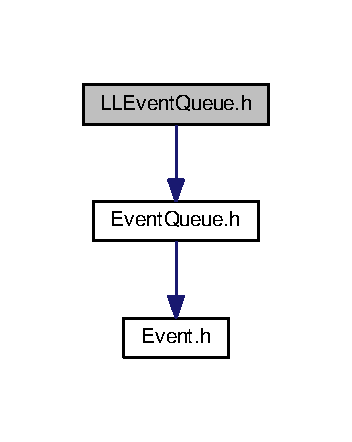
\includegraphics[width=169pt]{_l_l_event_queue_8h__incl}
\end{center}
\end{figure}
This graph shows which files directly or indirectly include this file\+:
\nopagebreak
\begin{figure}[H]
\begin{center}
\leavevmode
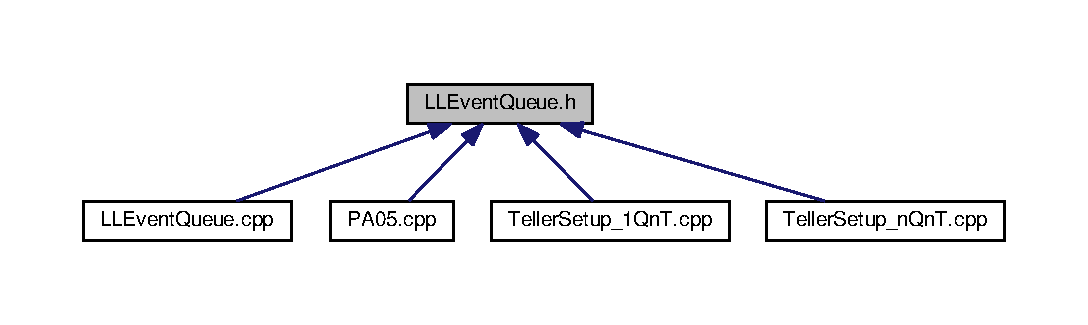
\includegraphics[width=350pt]{_l_l_event_queue_8h__dep__incl}
\end{center}
\end{figure}
\subsection*{Classes}
\begin{DoxyCompactItemize}
\item 
struct \hyperlink{struct_l_l_e_q_node}{L\+L\+E\+Q\+Node}
\begin{DoxyCompactList}\small\item\em A node in an \hyperlink{class_l_l_event_queue}{L\+L\+Event\+Queue}. \end{DoxyCompactList}\item 
class \hyperlink{class_l_l_event_queue}{L\+L\+Event\+Queue}
\begin{DoxyCompactList}\small\item\em A Linked-\/\+List-\/\+Based \hyperlink{struct_event}{Event} Queue. \end{DoxyCompactList}\end{DoxyCompactItemize}


\subsection{Detailed Description}
Declares the Linked-\/\+List-\/\+Based \hyperlink{struct_event}{Event} Queue class. 

\begin{DoxyAuthor}{Author}
Matthew Bauer 
\end{DoxyAuthor}

\hypertarget{_p_a05_8cpp}{}\section{P\+A05.\+cpp File Reference}
\label{_p_a05_8cpp}\index{P\+A05.\+cpp@{P\+A05.\+cpp}}


Main file for C\+S302/\+P\+A05.  


{\ttfamily \#include $<$fstream$>$}\\*
{\ttfamily \#include $<$iostream$>$}\\*
{\ttfamily \#include \char`\"{}Event.\+h\char`\"{}}\\*
{\ttfamily \#include \char`\"{}A\+B\+Event\+Queue.\+h\char`\"{}}\\*
{\ttfamily \#include \char`\"{}L\+L\+Event\+Queue.\+h\char`\"{}}\\*
{\ttfamily \#include \char`\"{}Teller\+Setup\+\_\+1\+Qn\+T.\+h\char`\"{}}\\*
{\ttfamily \#include \char`\"{}Teller\+Setup\+\_\+n\+Qn\+T.\+h\char`\"{}}\\*
Include dependency graph for P\+A05.\+cpp\+:
\nopagebreak
\begin{figure}[H]
\begin{center}
\leavevmode
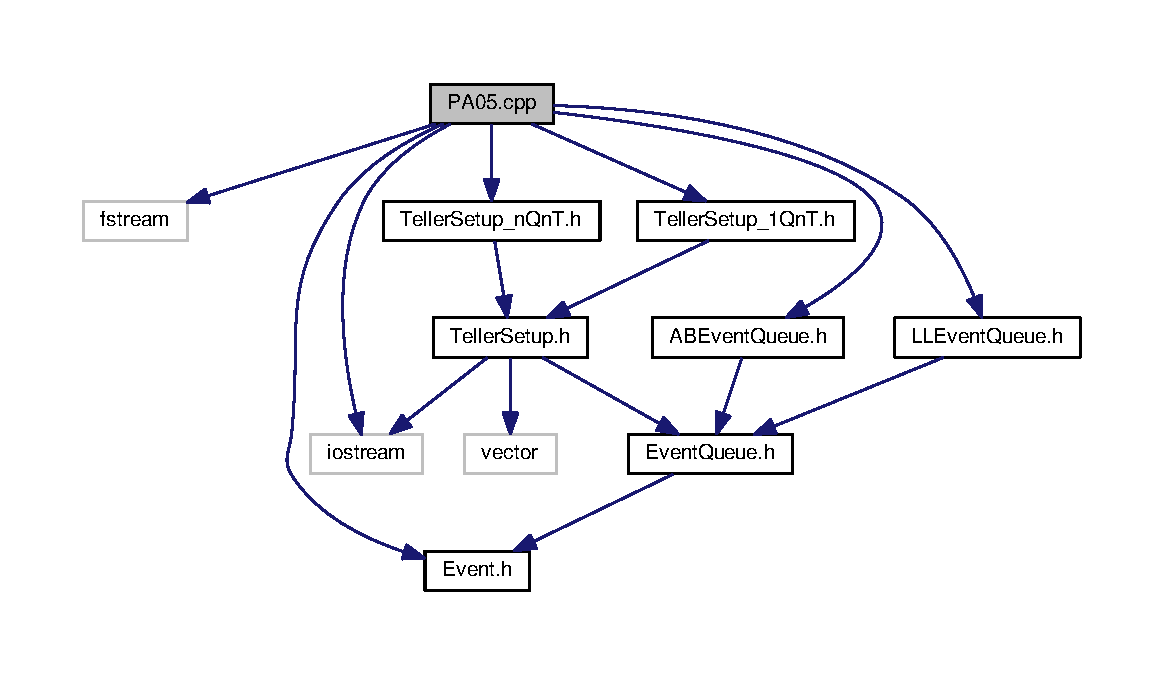
\includegraphics[width=350pt]{_p_a05_8cpp__incl}
\end{center}
\end{figure}
\subsection*{Functions}
\begin{DoxyCompactItemize}
\item 
void \hyperlink{_p_a05_8cpp_a41b59b08be156a44fb1d0d69c2d3d606}{Test\+Setup} (\hyperlink{class_teller_setup}{Teller\+Setup} $\ast$setup, std\+::ostream \&out)
\begin{DoxyCompactList}\small\item\em Test the given \hyperlink{class_teller_setup}{Teller\+Setup} on 10 samples. \end{DoxyCompactList}\item 
int \hyperlink{_p_a05_8cpp_ae66f6b31b5ad750f1fe042a706a4e3d4}{main} ()
\begin{DoxyCompactList}\small\item\em Program entry point. \end{DoxyCompactList}\end{DoxyCompactItemize}
\subsection*{Variables}
\begin{DoxyCompactItemize}
\item 
const int \hyperlink{_p_a05_8cpp_a5da6d9ec042926de0511396589d1a77a}{N\+U\+M\+\_\+\+E\+V\+E\+N\+TS} = 99999
\begin{DoxyCompactList}\small\item\em The number of events to use per simulation. \end{DoxyCompactList}\item 
const int \hyperlink{_p_a05_8cpp_aa39d0f8ca69f2dceb1efdb2c8030e34a}{M\+I\+N\+\_\+\+A\+R\+R\+I\+V\+AL} = 0
\item 
const int \hyperlink{_p_a05_8cpp_a39c92f8642d5e116d10a3c45fc60a2c3}{M\+A\+X\+\_\+\+A\+R\+R\+I\+V\+AL} = 100000
\item 
const int \hyperlink{_p_a05_8cpp_af00d30c4c9cd2a4bcd0cb0084bcabd30}{M\+I\+N\+\_\+\+D\+U\+R\+A\+T\+I\+ON} = 1
\item 
const int \hyperlink{_p_a05_8cpp_a2564fde0b4c94421653b40a37597aa62}{M\+A\+X\+\_\+\+D\+U\+R\+A\+T\+I\+ON} = 100
\end{DoxyCompactItemize}


\subsection{Detailed Description}
Main file for C\+S302/\+P\+A05. 

\begin{DoxyAuthor}{Author}
Matthew Bauer 
\end{DoxyAuthor}


\subsection{Function Documentation}
\index{P\+A05.\+cpp@{P\+A05.\+cpp}!main@{main}}
\index{main@{main}!P\+A05.\+cpp@{P\+A05.\+cpp}}
\subsubsection[{\texorpdfstring{main()}{main()}}]{\setlength{\rightskip}{0pt plus 5cm}int main (
\begin{DoxyParamCaption}
{}
\end{DoxyParamCaption}
)}\hypertarget{_p_a05_8cpp_ae66f6b31b5ad750f1fe042a706a4e3d4}{}\label{_p_a05_8cpp_ae66f6b31b5ad750f1fe042a706a4e3d4}


Program entry point. 

\index{P\+A05.\+cpp@{P\+A05.\+cpp}!Test\+Setup@{Test\+Setup}}
\index{Test\+Setup@{Test\+Setup}!P\+A05.\+cpp@{P\+A05.\+cpp}}
\subsubsection[{\texorpdfstring{Test\+Setup(\+Teller\+Setup $\ast$setup, std\+::ostream \&out)}{TestSetup(TellerSetup *setup, std::ostream &out)}}]{\setlength{\rightskip}{0pt plus 5cm}void Test\+Setup (
\begin{DoxyParamCaption}
\item[{{\bf Teller\+Setup} $\ast$}]{setup, }
\item[{std\+::ostream \&}]{out}
\end{DoxyParamCaption}
)}\hypertarget{_p_a05_8cpp_a41b59b08be156a44fb1d0d69c2d3d606}{}\label{_p_a05_8cpp_a41b59b08be156a44fb1d0d69c2d3d606}


Test the given \hyperlink{class_teller_setup}{Teller\+Setup} on 10 samples. 

Uses array-\/based queues. 
\begin{DoxyParams}{Parameters}
{\em p\+EvQ} & A pointer to the \hyperlink{class_event_queue}{Event\+Queue} to test. \\
\hline
{\em out} & The stream to send output to. \\
\hline
\end{DoxyParams}


\subsection{Variable Documentation}
\index{P\+A05.\+cpp@{P\+A05.\+cpp}!M\+A\+X\+\_\+\+A\+R\+R\+I\+V\+AL@{M\+A\+X\+\_\+\+A\+R\+R\+I\+V\+AL}}
\index{M\+A\+X\+\_\+\+A\+R\+R\+I\+V\+AL@{M\+A\+X\+\_\+\+A\+R\+R\+I\+V\+AL}!P\+A05.\+cpp@{P\+A05.\+cpp}}
\subsubsection[{\texorpdfstring{M\+A\+X\+\_\+\+A\+R\+R\+I\+V\+AL}{MAX_ARRIVAL}}]{\setlength{\rightskip}{0pt plus 5cm}const int M\+A\+X\+\_\+\+A\+R\+R\+I\+V\+AL = 100000}\hypertarget{_p_a05_8cpp_a39c92f8642d5e116d10a3c45fc60a2c3}{}\label{_p_a05_8cpp_a39c92f8642d5e116d10a3c45fc60a2c3}
\index{P\+A05.\+cpp@{P\+A05.\+cpp}!M\+A\+X\+\_\+\+D\+U\+R\+A\+T\+I\+ON@{M\+A\+X\+\_\+\+D\+U\+R\+A\+T\+I\+ON}}
\index{M\+A\+X\+\_\+\+D\+U\+R\+A\+T\+I\+ON@{M\+A\+X\+\_\+\+D\+U\+R\+A\+T\+I\+ON}!P\+A05.\+cpp@{P\+A05.\+cpp}}
\subsubsection[{\texorpdfstring{M\+A\+X\+\_\+\+D\+U\+R\+A\+T\+I\+ON}{MAX_DURATION}}]{\setlength{\rightskip}{0pt plus 5cm}const int M\+A\+X\+\_\+\+D\+U\+R\+A\+T\+I\+ON = 100}\hypertarget{_p_a05_8cpp_a2564fde0b4c94421653b40a37597aa62}{}\label{_p_a05_8cpp_a2564fde0b4c94421653b40a37597aa62}
\index{P\+A05.\+cpp@{P\+A05.\+cpp}!M\+I\+N\+\_\+\+A\+R\+R\+I\+V\+AL@{M\+I\+N\+\_\+\+A\+R\+R\+I\+V\+AL}}
\index{M\+I\+N\+\_\+\+A\+R\+R\+I\+V\+AL@{M\+I\+N\+\_\+\+A\+R\+R\+I\+V\+AL}!P\+A05.\+cpp@{P\+A05.\+cpp}}
\subsubsection[{\texorpdfstring{M\+I\+N\+\_\+\+A\+R\+R\+I\+V\+AL}{MIN_ARRIVAL}}]{\setlength{\rightskip}{0pt plus 5cm}const int M\+I\+N\+\_\+\+A\+R\+R\+I\+V\+AL = 0}\hypertarget{_p_a05_8cpp_aa39d0f8ca69f2dceb1efdb2c8030e34a}{}\label{_p_a05_8cpp_aa39d0f8ca69f2dceb1efdb2c8030e34a}
\index{P\+A05.\+cpp@{P\+A05.\+cpp}!M\+I\+N\+\_\+\+D\+U\+R\+A\+T\+I\+ON@{M\+I\+N\+\_\+\+D\+U\+R\+A\+T\+I\+ON}}
\index{M\+I\+N\+\_\+\+D\+U\+R\+A\+T\+I\+ON@{M\+I\+N\+\_\+\+D\+U\+R\+A\+T\+I\+ON}!P\+A05.\+cpp@{P\+A05.\+cpp}}
\subsubsection[{\texorpdfstring{M\+I\+N\+\_\+\+D\+U\+R\+A\+T\+I\+ON}{MIN_DURATION}}]{\setlength{\rightskip}{0pt plus 5cm}const int M\+I\+N\+\_\+\+D\+U\+R\+A\+T\+I\+ON = 1}\hypertarget{_p_a05_8cpp_af00d30c4c9cd2a4bcd0cb0084bcabd30}{}\label{_p_a05_8cpp_af00d30c4c9cd2a4bcd0cb0084bcabd30}
\index{P\+A05.\+cpp@{P\+A05.\+cpp}!N\+U\+M\+\_\+\+E\+V\+E\+N\+TS@{N\+U\+M\+\_\+\+E\+V\+E\+N\+TS}}
\index{N\+U\+M\+\_\+\+E\+V\+E\+N\+TS@{N\+U\+M\+\_\+\+E\+V\+E\+N\+TS}!P\+A05.\+cpp@{P\+A05.\+cpp}}
\subsubsection[{\texorpdfstring{N\+U\+M\+\_\+\+E\+V\+E\+N\+TS}{NUM_EVENTS}}]{\setlength{\rightskip}{0pt plus 5cm}const int N\+U\+M\+\_\+\+E\+V\+E\+N\+TS = 99999}\hypertarget{_p_a05_8cpp_a5da6d9ec042926de0511396589d1a77a}{}\label{_p_a05_8cpp_a5da6d9ec042926de0511396589d1a77a}


The number of events to use per simulation. 


\hypertarget{_teller_setup_8cpp}{}\section{Teller\+Setup.\+cpp File Reference}
\label{_teller_setup_8cpp}\index{Teller\+Setup.\+cpp@{Teller\+Setup.\+cpp}}
{\ttfamily \#include \char`\"{}Teller\+Setup.\+h\char`\"{}}\\*
{\ttfamily \#include $<$stdarg.\+h$>$}\\*
{\ttfamily \#include $<$iostream$>$}\\*
Include dependency graph for Teller\+Setup.\+cpp\+:
\nopagebreak
\begin{figure}[H]
\begin{center}
\leavevmode
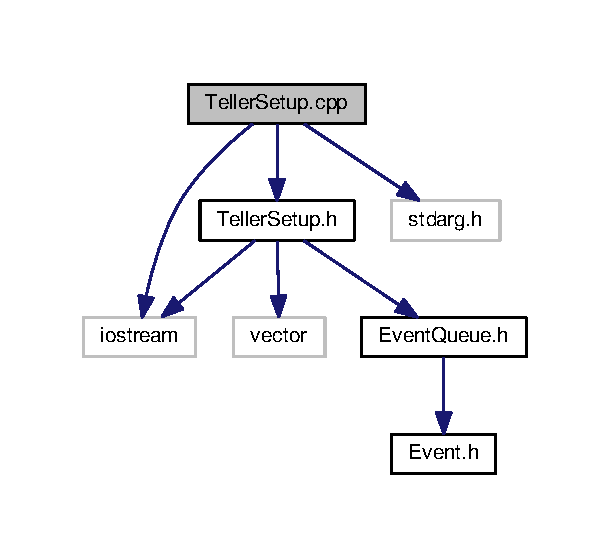
\includegraphics[width=293pt]{_teller_setup_8cpp__incl}
\end{center}
\end{figure}
\subsection*{Functions}
\begin{DoxyCompactItemize}
\item 
int \hyperlink{_teller_setup_8cpp_ae065b9357496e41e5ca7db6df6287b82}{get\+Earliest\+Time} (const std\+::vector$<$ int $>$ \&times)
\begin{DoxyCompactList}\small\item\em Take the min of the given numbers, with -\/1 values excluded. \end{DoxyCompactList}\end{DoxyCompactItemize}


\subsection{Function Documentation}
\index{Teller\+Setup.\+cpp@{Teller\+Setup.\+cpp}!get\+Earliest\+Time@{get\+Earliest\+Time}}
\index{get\+Earliest\+Time@{get\+Earliest\+Time}!Teller\+Setup.\+cpp@{Teller\+Setup.\+cpp}}
\subsubsection[{\texorpdfstring{get\+Earliest\+Time(const std\+::vector$<$ int $>$ \&times)}{getEarliestTime(const std::vector< int > &times)}}]{\setlength{\rightskip}{0pt plus 5cm}int get\+Earliest\+Time (
\begin{DoxyParamCaption}
\item[{const std\+::vector$<$ int $>$ \&}]{times}
\end{DoxyParamCaption}
)}\hypertarget{_teller_setup_8cpp_ae065b9357496e41e5ca7db6df6287b82}{}\label{_teller_setup_8cpp_ae065b9357496e41e5ca7db6df6287b82}


Take the min of the given numbers, with -\/1 values excluded. 

For use by \hyperlink{class_teller_setup}{Teller\+Setup}. 
\begin{DoxyParams}{Parameters}
{\em times} & The times. \\
\hline
\end{DoxyParams}

\hypertarget{_teller_setup_8h}{}\section{Teller\+Setup.\+h File Reference}
\label{_teller_setup_8h}\index{Teller\+Setup.\+h@{Teller\+Setup.\+h}}


Declares the \hyperlink{class_teller_setup}{Teller\+Setup} abstract class.  


{\ttfamily \#include $<$iostream$>$}\\*
{\ttfamily \#include $<$vector$>$}\\*
{\ttfamily \#include \char`\"{}Event\+Queue.\+h\char`\"{}}\\*
Include dependency graph for Teller\+Setup.\+h\+:
\nopagebreak
\begin{figure}[H]
\begin{center}
\leavevmode
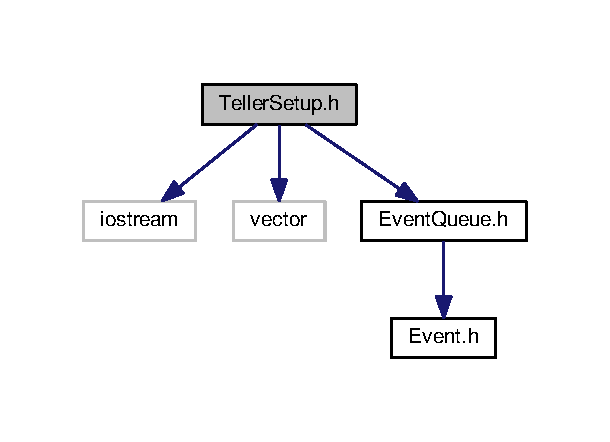
\includegraphics[width=293pt]{_teller_setup_8h__incl}
\end{center}
\end{figure}
This graph shows which files directly or indirectly include this file\+:
\nopagebreak
\begin{figure}[H]
\begin{center}
\leavevmode
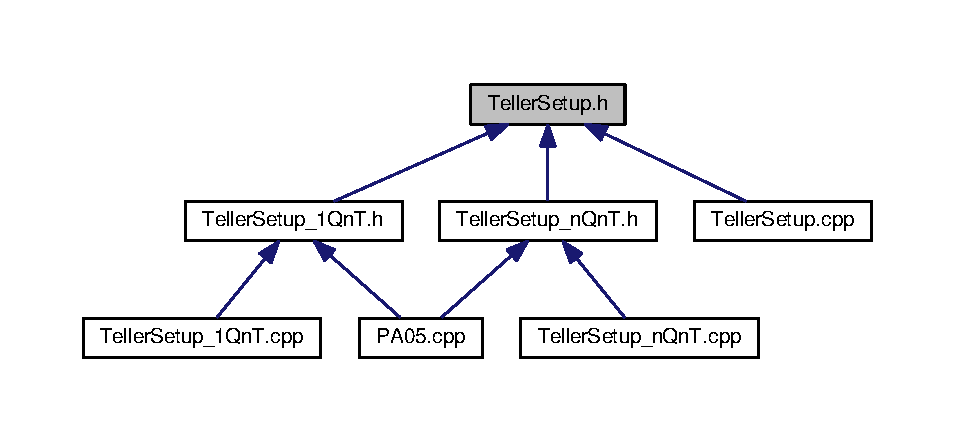
\includegraphics[width=350pt]{_teller_setup_8h__dep__incl}
\end{center}
\end{figure}
\subsection*{Classes}
\begin{DoxyCompactItemize}
\item 
class \hyperlink{class_teller_setup}{Teller\+Setup}
\item 
class \hyperlink{class_tickable}{Tickable}
\begin{DoxyCompactList}\small\item\em A \hyperlink{class_tickable}{Tickable} object. \end{DoxyCompactList}\item 
class \hyperlink{class_teller}{Teller}
\begin{DoxyCompactList}\small\item\em Models a bank teller. \end{DoxyCompactList}\item 
class \hyperlink{class_tickable_queue}{Tickable\+Queue}
\begin{DoxyCompactList}\small\item\em An \hyperlink{class_event_queue}{Event\+Queue} wrapper that enables tick functionality. \end{DoxyCompactList}\end{DoxyCompactItemize}
\subsection*{Functions}
\begin{DoxyCompactItemize}
\item 
int \hyperlink{_teller_setup_8h_ae065b9357496e41e5ca7db6df6287b82}{get\+Earliest\+Time} (const std\+::vector$<$ int $>$ \&times)
\begin{DoxyCompactList}\small\item\em Take the min of the given numbers, with -\/1 values excluded. \end{DoxyCompactList}\end{DoxyCompactItemize}


\subsection{Detailed Description}
Declares the \hyperlink{class_teller_setup}{Teller\+Setup} abstract class. 

\begin{DoxyAuthor}{Author}
Matthew Bauer 
\end{DoxyAuthor}


\subsection{Function Documentation}
\index{Teller\+Setup.\+h@{Teller\+Setup.\+h}!get\+Earliest\+Time@{get\+Earliest\+Time}}
\index{get\+Earliest\+Time@{get\+Earliest\+Time}!Teller\+Setup.\+h@{Teller\+Setup.\+h}}
\subsubsection[{\texorpdfstring{get\+Earliest\+Time(const std\+::vector$<$ int $>$ \&times)}{getEarliestTime(const std::vector< int > &times)}}]{\setlength{\rightskip}{0pt plus 5cm}int get\+Earliest\+Time (
\begin{DoxyParamCaption}
\item[{const std\+::vector$<$ int $>$ \&}]{times}
\end{DoxyParamCaption}
)}\hypertarget{_teller_setup_8h_ae065b9357496e41e5ca7db6df6287b82}{}\label{_teller_setup_8h_ae065b9357496e41e5ca7db6df6287b82}


Take the min of the given numbers, with -\/1 values excluded. 

For use by \hyperlink{class_teller_setup}{Teller\+Setup}. 
\begin{DoxyParams}{Parameters}
{\em times} & The times. \\
\hline
\end{DoxyParams}

\hypertarget{_teller_setup__1_qn_t_8cpp}{}\section{Teller\+Setup\+\_\+1\+Qn\+T.\+cpp File Reference}
\label{_teller_setup__1_qn_t_8cpp}\index{Teller\+Setup\+\_\+1\+Qn\+T.\+cpp@{Teller\+Setup\+\_\+1\+Qn\+T.\+cpp}}
{\ttfamily \#include \char`\"{}Teller\+Setup\+\_\+1\+Qn\+T.\+h\char`\"{}}\\*
{\ttfamily \#include \char`\"{}L\+L\+Event\+Queue.\+h\char`\"{}}\\*
{\ttfamily \#include $<$chrono$>$}\\*
{\ttfamily \#include $<$iostream$>$}\\*
Include dependency graph for Teller\+Setup\+\_\+1\+Qn\+T.\+cpp\+:
\nopagebreak
\begin{figure}[H]
\begin{center}
\leavevmode
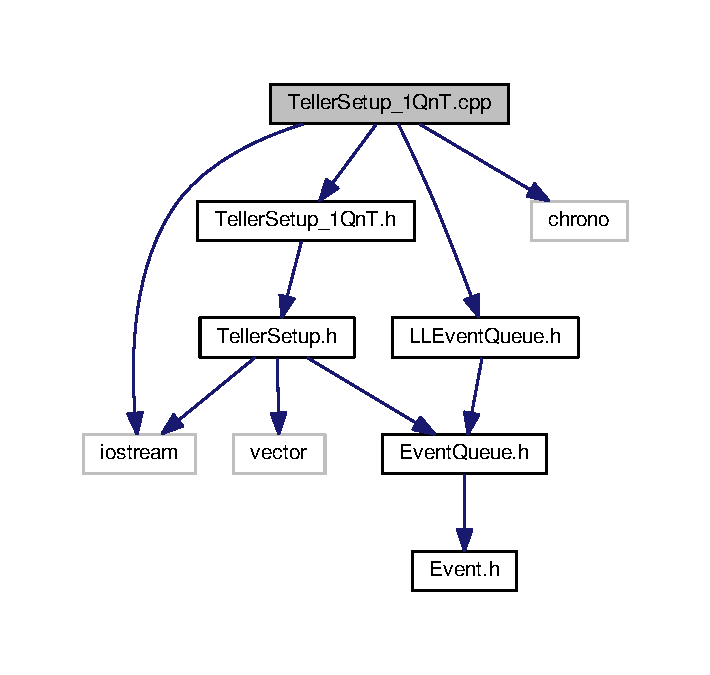
\includegraphics[width=341pt]{_teller_setup__1_qn_t_8cpp__incl}
\end{center}
\end{figure}

\hypertarget{_teller_setup__1_qn_t_8h}{}\section{Teller\+Setup\+\_\+1\+Qn\+T.\+h File Reference}
\label{_teller_setup__1_qn_t_8h}\index{Teller\+Setup\+\_\+1\+Qn\+T.\+h@{Teller\+Setup\+\_\+1\+Qn\+T.\+h}}


Declares a \hyperlink{class_teller_setup}{Teller\+Setup} with 1 Queue and N Tellers.  


{\ttfamily \#include \char`\"{}Teller\+Setup.\+h\char`\"{}}\\*
Include dependency graph for Teller\+Setup\+\_\+1\+Qn\+T.\+h\+:
\nopagebreak
\begin{figure}[H]
\begin{center}
\leavevmode
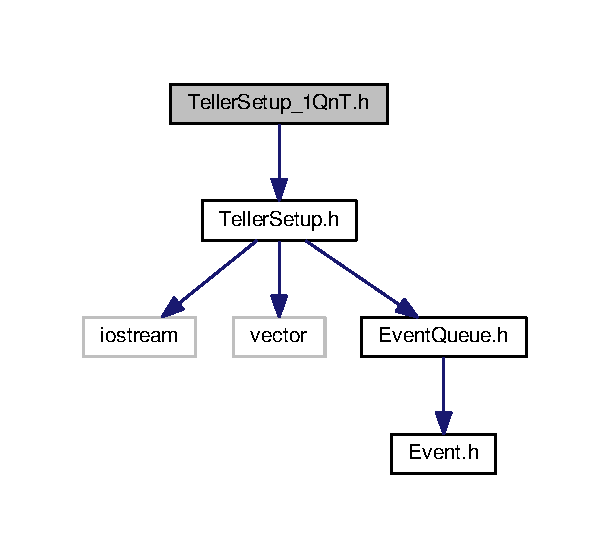
\includegraphics[width=293pt]{_teller_setup__1_qn_t_8h__incl}
\end{center}
\end{figure}
This graph shows which files directly or indirectly include this file\+:
\nopagebreak
\begin{figure}[H]
\begin{center}
\leavevmode
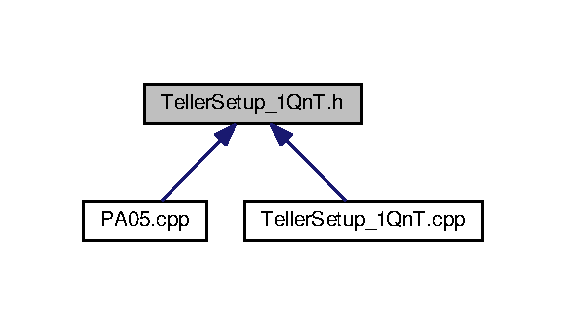
\includegraphics[width=272pt]{_teller_setup__1_qn_t_8h__dep__incl}
\end{center}
\end{figure}
\subsection*{Classes}
\begin{DoxyCompactItemize}
\item 
class \hyperlink{class_teller_setup__1_qn_t}{Teller\+Setup\+\_\+1\+QnT}
\end{DoxyCompactItemize}


\subsection{Detailed Description}
Declares a \hyperlink{class_teller_setup}{Teller\+Setup} with 1 Queue and N Tellers. 

\begin{DoxyAuthor}{Author}
Matthew Bauer 
\end{DoxyAuthor}

\hypertarget{_teller_setup__n_qn_t_8cpp}{}\section{Teller\+Setup\+\_\+n\+Qn\+T.\+cpp File Reference}
\label{_teller_setup__n_qn_t_8cpp}\index{Teller\+Setup\+\_\+n\+Qn\+T.\+cpp@{Teller\+Setup\+\_\+n\+Qn\+T.\+cpp}}
{\ttfamily \#include \char`\"{}Teller\+Setup\+\_\+n\+Qn\+T.\+h\char`\"{}}\\*
{\ttfamily \#include \char`\"{}L\+L\+Event\+Queue.\+h\char`\"{}}\\*
{\ttfamily \#include $<$chrono$>$}\\*
Include dependency graph for Teller\+Setup\+\_\+n\+Qn\+T.\+cpp\+:
\nopagebreak
\begin{figure}[H]
\begin{center}
\leavevmode
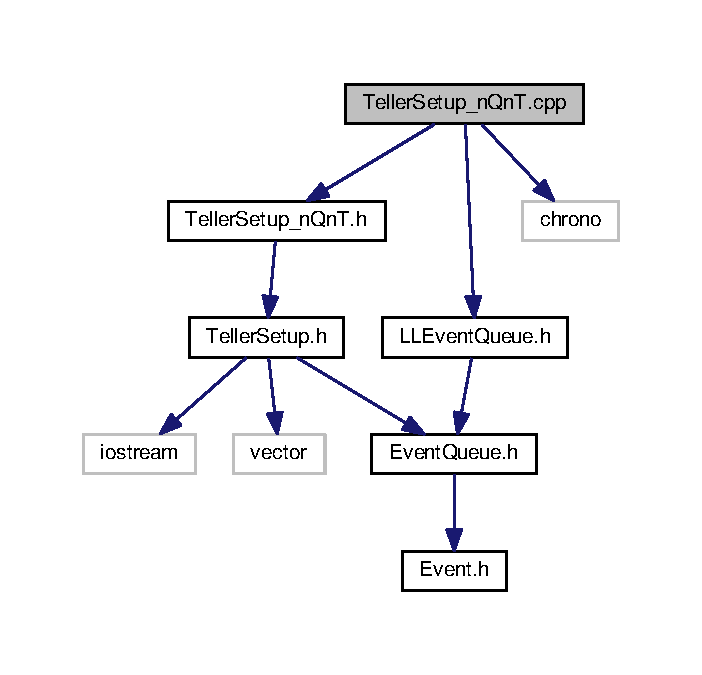
\includegraphics[width=337pt]{_teller_setup__n_qn_t_8cpp__incl}
\end{center}
\end{figure}

\hypertarget{_teller_setup__n_qn_t_8h}{}\section{Teller\+Setup\+\_\+n\+Qn\+T.\+h File Reference}
\label{_teller_setup__n_qn_t_8h}\index{Teller\+Setup\+\_\+n\+Qn\+T.\+h@{Teller\+Setup\+\_\+n\+Qn\+T.\+h}}


Declares a \hyperlink{class_teller_setup}{Teller\+Setup} with N Queues and N Tellers.  


{\ttfamily \#include \char`\"{}Teller\+Setup.\+h\char`\"{}}\\*
Include dependency graph for Teller\+Setup\+\_\+n\+Qn\+T.\+h\+:
\nopagebreak
\begin{figure}[H]
\begin{center}
\leavevmode
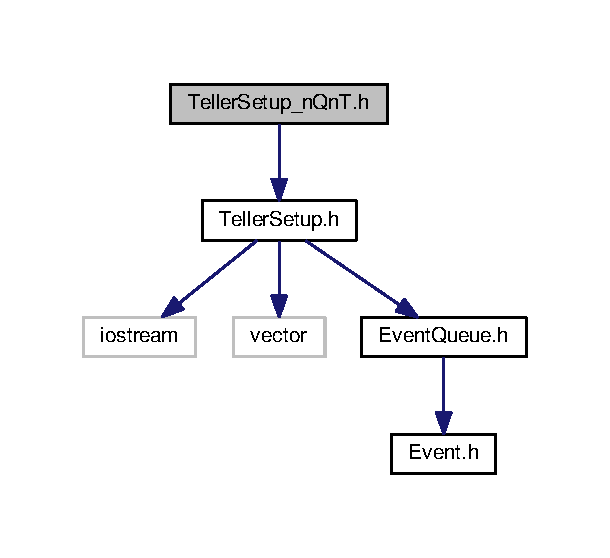
\includegraphics[width=293pt]{_teller_setup__n_qn_t_8h__incl}
\end{center}
\end{figure}
This graph shows which files directly or indirectly include this file\+:
\nopagebreak
\begin{figure}[H]
\begin{center}
\leavevmode
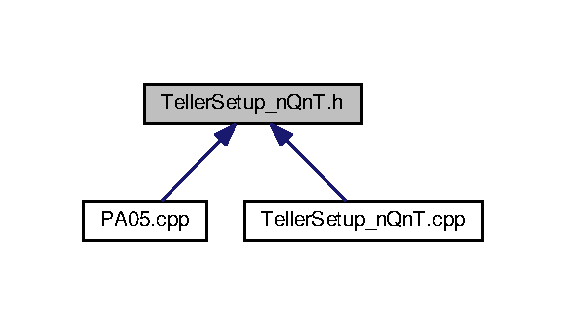
\includegraphics[width=272pt]{_teller_setup__n_qn_t_8h__dep__incl}
\end{center}
\end{figure}
\subsection*{Classes}
\begin{DoxyCompactItemize}
\item 
class \hyperlink{class_teller_setup__n_qn_t}{Teller\+Setup\+\_\+n\+QnT}
\end{DoxyCompactItemize}


\subsection{Detailed Description}
Declares a \hyperlink{class_teller_setup}{Teller\+Setup} with N Queues and N Tellers. 

\begin{DoxyAuthor}{Author}
Matthew Bauer 
\end{DoxyAuthor}

%--- End generated contents ---

% Index
\backmatter
\newpage
\phantomsection
\clearemptydoublepage
\addcontentsline{toc}{chapter}{Index}
\printindex

\end{document}
